%%%%%%%%%%%%%%%%%%%%%%%%%%%%%%%%%%%%%%%%%%%%%%%%%%%%%%%%%%%%%%%%%%
%%%%%%%% ICML 2012 EXAMPLE LATEX SUBMISSION FILE %%%%%%%%%%%%%%%%%
%%%%%%%%%%%%%%%%%%%%%%%%%%%%%%%%%%%%%%%%%%%%%%%%%%%%%%%%%%%%%%%%%%

% Use the following line _only_ if you're still using LaTeX 2.09.
%\documentstyle[icml2012,epsf,natbib]{article}
% If you rely on Latex2e packages, like most moden people use this:

\documentclass{article}

% For figures
\usepackage{graphicx} % more modern
\usepackage[caption=false]{subfig}

%\usepackage{epsfig} % less modern
%\usepackage{subfigure} 

% For citations
\usepackage{natbib}

% For algorithms
\usepackage{algorithm}
\usepackage{algorithmic}

% For font
\usepackage{amssymb}

% For math equations
\usepackage{mathtools}

% For references
%\usepackage{nature}

% As of 2011, we use the hyperref package to produce hyperlinks in the
% resulting PDF.  If this breaks your system, please commend out the
% following usepackage line and replace \usepackage{icml2012} with
% \usepackage[nohyperref]{icml2012} above.
\usepackage{hyperref}

% Packages hyperref and algorithmic misbehave sometimes.  We can fix
% this with the following command.
\newcommand{\theHalgorithm}{\arabic{algorithm}}

% Employ the following version of the ``usepackage'' statement for
% submitting the draft version of the paper for review.  This will set
% the note in the first column to ``Under review.  Do not distribute.''
%\usepackage{icml2012} 
% Employ this version of the ``usepackage'' statement after the paper has
% been accepted, when creating the final version.  This will set the
% note in the first column to ``Appearing in''
 \usepackage[accepted]{icml2012}


% The \icmltitle you define below is probably too long as a header.
% Therefore, a short form for the running title is supplied here:
\icmltitlerunning{2D Visualization of Immune System Cellular Protein Data by Nonlinear Dimensionality Reduction}

\begin{document} 

\twocolumn[
\icmltitle{2D Visualization of Immune System Cellular Protein Data by Nonlinear Dimensionality Reduction}

% Author Information
\icmlauthor{Andre Esteva}{esteva@stanford.edu}
\icmladdress{Stanford University, Electrical Engineering, 496 Lomita Mall, Durand 196, Stanford, CA 94305 USA}            

\icmlauthor{Anand Sampat}{asampat@stanford.edu}
\icmladdress{Stanford University, Electrical Engineering, 450 Serra Mall, Stanford, CA 94305 USA}

\icmlauthor{Amit Badlani}{abadlani@stanford.edu}
\icmladdress{Stanford University, Electrical Engineering, 450 Serra Mall, Stanford, CA 94305 USA}

% You may provide any keywords that you 
% find helpful for describing your paper; these are used to populate 
% the "keywords" metadata in the PDF but will not be shown in the document
\icmlkeywords{dimensionality reduction, cancer data, stochastic neighbor embedding (SNE), machine learning, CS229}

\vskip 0.3in
]

% ABSTRACT
\begin{abstract} 
We present in this paper a way to effectively visualize multi-dimensional immune system cellular data by means of nonlinear methods. We find that Stochastic Neighbor Embedding (SNE), and it's variations, t-SNE and s-SNE, to be most effective at successfully mapping clusters of points into a two dimensional embedding space while preserving both the structure between similar points and the disparity between different clusters. Using a centroid-based metric that relabels points according to the cluster centroid to which they are closest, we conclude that SNE works significantly better than linear and spectral methods. In addtional, by using an optimization approach for SNE similar to Newton's Method, but with the Hessian of the objective function, $\nabla ^2 (E) $, replaced by its first term, we are able to run the SNE varients and EE two orders of magnitude faster than with standard optimization.

\end{abstract} 

% INTRO
\section{Introduction}
\label{intro}

\subsection{Immune Cell Data}

In the field of cancer immunology, scientists use the protein content of immune system cells as a way to identify a cells corresponding type. For example, immune system cells, which are contained in bone marrow, are comprised of a variety of cell types, and to a large degree are uniquely identifiable by the proteins they contain. Highly sophisticated methods have been developed that process cells and return information on the types and quantities of proteins expressed in those cells. This data can then be viewed by an expert in the field and categorized. The laborious process of viewing the different dimensions of protein expression and categorizing a cell's type is known as gating. Figure ~\ref{CellGating}, below, taken from \cite{Amir:2013jp} shows this graphically.

\begin{figure}[ht]
\label{CellGating}
\vskip 0.2in
\begin{center}
\centerline{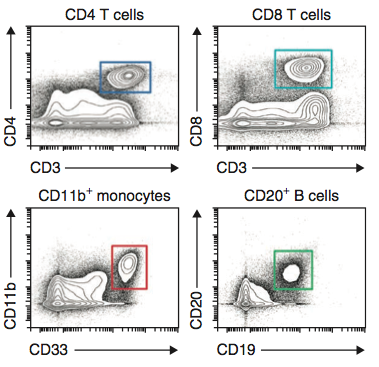
\includegraphics[width=\columnwidth]{CellGating}}
\caption{Strategy for cell gating: Two single dimensions of a cell are viewed at a time
and through an iterative process the cell is classified}
\end{center}
\vskip -0.2in
\end{figure} 

\subsection{Project Goals and Metrics}

It is of interest to cancer immunologists to find structure within multi-dimensional protein expression space and map it onto a lower dimensions (refered to henceforth as a map space) for ease of visualization and understanding. As cells change and evolve, so too do the types and quantities of the proteins they express. This leads to a shifting of their representation in multi-dimensional space which can be tracked. Dimensionality reduction of original biological data coupled with a metric for how well the projection represents the original data would provide biologists with a powerful tool for understanding the structure of their data. To address these challenges we demonstrate:

\begin{itemize}
\item The application of linear and non-linear methods of dimensionality reduction of multi-dimensional protein data
\item A metric-based comparison of how each algorithm performs
\end{itemize}

% DATA REPRESENTATION
\section{Data Representation}
\label{data_representation}

\subsection{Data Acquisition}

\textbf{Mass cytometry} is a single-cell multiparametric protein detection technology based on inductively coupled plasma mass spectrometry. It is an extension of flow cytometry in which antibodies are tagged with isotopically pure rare earth elements allowing simultaneous measurement of greater than 40 parameters while circumventing the issue of spectral overlap. In single-cell droplet form, the cells are passed through an elemental mass spectrometer and an integrator to generate an $m \times p$ matrix where $m$ is the number of cells processed and $p$ is the number of distinct proteins contained in the cell set. These matrices are stored as .FCS files in online databanks which we have been granted access to. Figure ~\ref{dataacquisition} shows this process. 

\begin{figure}[ht]
\vskip 0.2in
\begin{center}
\centerline{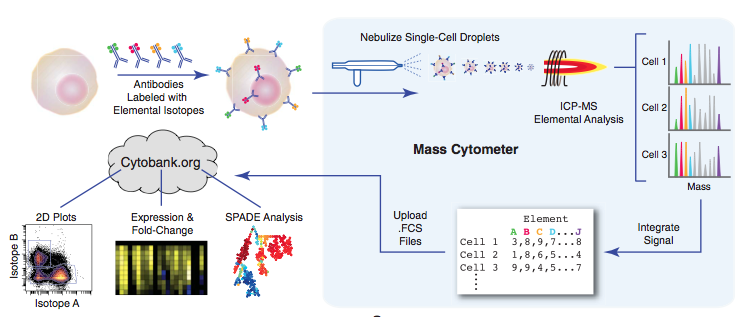
\includegraphics[width=\columnwidth]{DataAcquisition}}
\caption{Overview of data acquisition, from extraction of cellular protein counts to storage in online databanks}
\end{center}
\label{dataacquisition}
\vskip -0.2in
\end{figure} 

Table ~\ref{table_cell_type} lists the cell types and subtypes that are parsed using this method. 

\begin{table}[tb]
\caption{Classification of Cell Types and their Corresponding Sub-Types}
\label{table_cell_type}
\vskip 0.15in
\begin{center}
\begin{small}
\begin{sc}
\begin{tabular}{lcccr}
\hline
\abovespace\belowspace
Cell Types & Sub-types  \\
\hline
\abovespace
Stem Cell	&  HSC, MPP, CMP, GMP, MEP \\
B Cells 	& Plasma, pre-B-I, pre-B- II, Immature, \\ 
		&			Mature CD38 low, Mature CD38 mid\\
T Cells	& Mature CD4+, Mature CD8+ \\
		& Naive CD4+, Naive CD8+  \\
NK		& -   \\
pDC		& - \\
\belowspace
Monocytes & CD11B - , CD11B high, CD11B mid \\
\hline
\end{tabular}
\end{sc}
\end{small}
\end{center}
\vskip -0.1in
\end{table}

\subsection{Feature Selection}
The $p=41$ protein counts collected for each cell that passes through mass cytometry is comprised of both intracellular and surface proteins. These two types play fundamentally different roles in cell identification. Surface proteins are semi-permanent markers that last for significant periods of time relative to the lifetime of a cell, whereas intracellular proteins are highly transient and can change quickly. This is analogous to classifying a person based on where they live (semi-permanent) versus what they wore on a particular day (transient). Understanding this, we select as our feature space the $n=17$ surface protein markers of the cell data.

% METHODS
\section{Methods}
\label{methods}

The datafiles provided contain cell counts on the order of tens of thousands where we consider each cell to be a point in $\mathbb{R}^n$. To simplify our algorithms and account for matrix size differences in the difference .FCS files we run our algorithms on equally sized portions of different cell data. In particular, if we let $\mathbb{S}$ be the set of all cell sub-types as defined in Table ~\ref{table_cell_type}, $S \in \mathbb{S}$  be some subset of interest with cardinality $|S|$, and N some fixed positive integer, then by taking N rows from each sub-type $s \in S$ we form a matrix $M \in \mathbb{R}^{N |S| \times n}$ on which we can run algorithms quickly and without giving unfair weighting to a particular cell sub-type.

We consider various algorithms which project sets of data in $\mathbb{R}^n$ onto $\mathbb{R}^2$ for easy visualization.

\subsection{Linear Methods}
Linear methods such as Principal Components Analysis (PCA) and multidimensional scaling are straightforward and standard ways of achieving dimensionality reduction. The caveat is the requirement that the data be linearly separable in the space being considered. Unlike SVMs, which have the ability to project data to higher dimensions in order to linearly separate it, PCA runs in the original dimension of the data. Given the nature of this data and the fact that cellular protein counts can vary largely between cell types, PCA is not an optimal method for visualizing these sorts of problems. We apply PCA and demonstrate that its visualization is quite poor, as expected.

\subsection{Spectral Methods}
Spectral methods like Locally Linear Embedding (LLE), ISOMAP, and Laplacian Eigenmaps (LE) seem like better candidates for dimensionality reduction of problems of this sort. For example, LE tries to preserve the local structure of the data while keeping the scale of the embedding data fixed, leading to good results on toy problems such as the swiss roll. We apply LLE and ISOMAP to this data set and show that the results are even worse than PCA.

\subsection{Nonlinear Methods}
Nonlinear methods, as demonstrated in the section below, are the most effective of the algorithms used for visualization of celllular protein data. Cellular protein data is largely believed to exist in multi-dimensional space in gaussian-distributed clumps that can have a high degree of overlap. These gaussians can exhibit high degrees of variation in their average and variance values. As such, we consider the variants of SNE, t-SNE and s-SNE, along with Elastic Embedding (EE) as prime candidates for effective visualization. These algorithms minimize objective functions that mimick attrack and repulsive forces in the mapping space, which keeps the images of nearby objects close while pushing all images apart from each other. They take the form $E(X, \lambda) = E^+(X) + \lambda E^-(X)$ where $E^+(X)$ is the attractive term, $E^-(X)$ the repulsive term, $\lambda \geq 0$ is a fixed parameter, and $X = \{x_n\}$ is the set of points in the mapping space. The repulsive term significantly improves them over spectral methods like LE. For comparison, we outline the objective functions $E$ of these algorithms.

Given two neighborhood graphs,
\begin{equation}
\label{wnm+}
w_{nm}^+ = exp(- \frac{1}{2} ||y_n - y_m||^2/\sigma^2) 
\end{equation}

\begin{equation}
\label{wnm-}
w_{nm}^- =||y_n - y_m||^2
\end{equation}

And conditional probability matrices $\{p_{nm}\}$ and $\{q_{nm}\}$ in both the original data space (points $y_n$) and mapping space (points $x_n$), respectively that a point selects any other point as its neighbor:

\begin{equation}
\label{pnm}
p_{nm} = \frac{\exp(-||y_n - y_m||^2/2\sigma^2)}{\sum_{k \neq n} \exp(-||y_n - y_m||^2/2\sigma^2)}
\end{equation}

\begin{equation}
\label{qnm}
q_{nm} = \frac{\exp(-||x_n - x_m||^2/2\sigma^2)}{\sum_{k \neq n} \exp(-||x_n - x_m||^2/2\sigma^2)}
\end{equation}

The objective functions for LE, SNE, t-SNE, s-SNE, and EE are given by, 

\begin{align*}
E_{LE}(X) &= \sum_{n,m=1}^N w_{nm} ||x_n - x_m||^2 \\
E_{SNE}(X) &= \sum_{n,m=1}^N p_{nm} ||x_n - x_m||^2 + \sum_{n=1}^N \log \sum_{m \neq n}^N \exp(-||x_n - x_m||^2) \\
E_{s-SNE}(X) &= \sum_{n,m=1}^N p_{nm} ||x_n - x_m||^2 + \log \sum_{n,m =1}^N \exp(-||x_n - x_m||^2) \\
E_{t-SNE}(X) &= \sum_{n,m=1}^N p_{nm} \log(1+||x_n - x_m||^2) \\ 
	&+ \sum_{n,m =1}^N (1 + ||-x_n - x_m||^2)^{-1} \\
E_{EE}(X) &= \sum_{n,m=1}^N w^+_{nm} ||x_n - x_m||^2 \\
	&+ \lambda \sum_{n,m =1}^N w^-_{nm} \exp (-||x_n - x_m||^2)
\end{align*}


\subsection{Fast Learning of Nonlinear Embeddings}
In order to speed up the SNE and EE algorithms, we employ a strategy for optimization of the objective functions in the "spectral direction" \cite{Vladymyrov:2012ws}. Optimization typically involves computing the gradient $g = \nabla E$ of the objective function and computing a descent direction as $p$ by solving the linear system $Bp = -g$ using some positive definitie $B$. When $B=I$ this is gradient descent, and for $B=\nabla^2 E$ we have Newton's Method. Descending in the spectral direction is accomplished by letting $B$ be the first term of $\nabla^2 E$ and, for small data sets (< 10,000 points) is two orders of magnitude faster than gradient descent and Newton's Method.

\subsection{Metric on Quality of Visualization}
We quantify the quality of the various algorithms at accurately segregating different cell types in the map space using a simple re-labeling technique. After projection, the averages of all the points (centroids) of each cell sub-type are calculated. Each point is then relabeled based on whichever centroid it is closest to. Formally, for cell sub-type $i$ with $P^{[i]}$ points $\{x^{[i]}\}$ in the projection space, the centroid is given by $\mu^{[i]} = \frac{1}{P^{[i]}} \sum_{j} x_j^{[i]}$, and each point $x$ is relabeled as sub-type $i = \arg \min_j ||\mu^{[j]} - x||$. The error of a visualization with $N$ points is then calculated as $err = \frac{1}{N} \sum_j^N 1\{\text{originalLabel}(x_j) \neq \text{newLabel}(x_j) \}$.

% RESULTS
\section{Results}

\subsection{Linear Methods - PCA}
We consider PCA over all 20 cell sub-types with 400 cells per cell sub-type and obtain a 62.18\% re-labeling error. Figure ~\ref{pca_plots_allcells} below shows the visualized data. It is clear that the overlap between points renders the map meaningless. The colored stars in the figures represent the centroids of each sub-type.

\begin{figure}[h]
\vskip 0.2in
%\centering
\begin{center}
\subfloat[Original Labels]{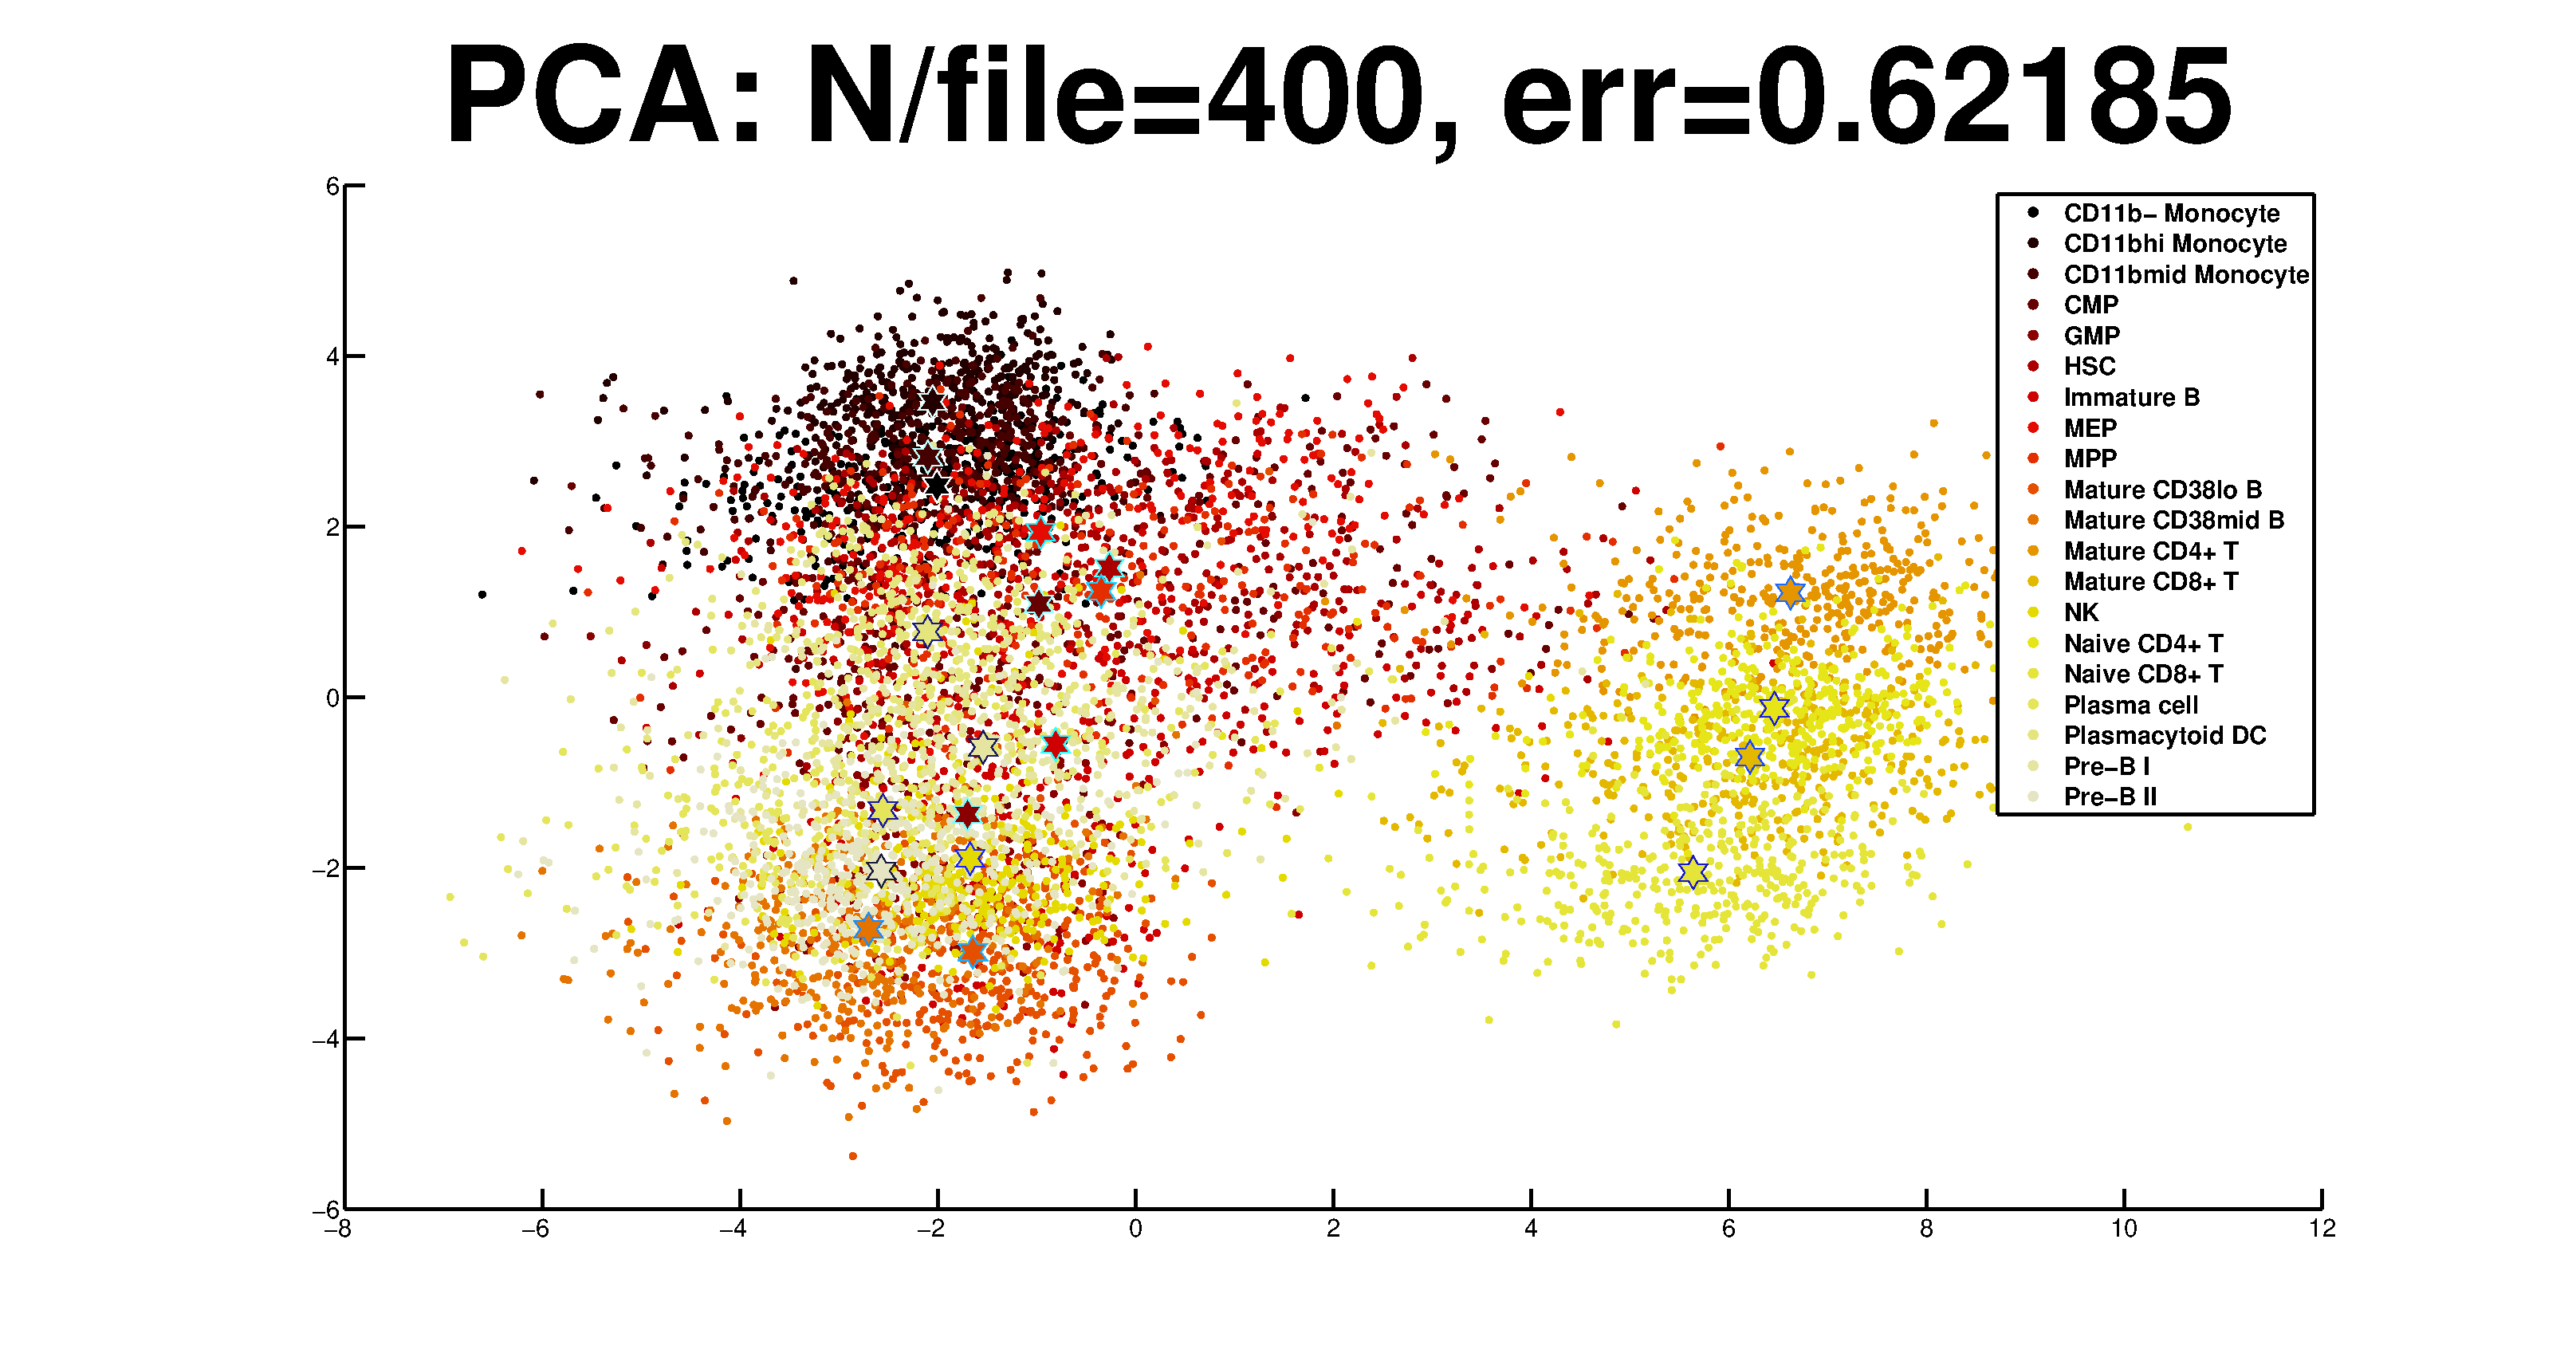
\includegraphics[width=0.47\columnwidth, trim = 2.5in 0.5in 1in 2in]{PCA_AllCells_N=400}}\quad
\subfloat[New Labels]{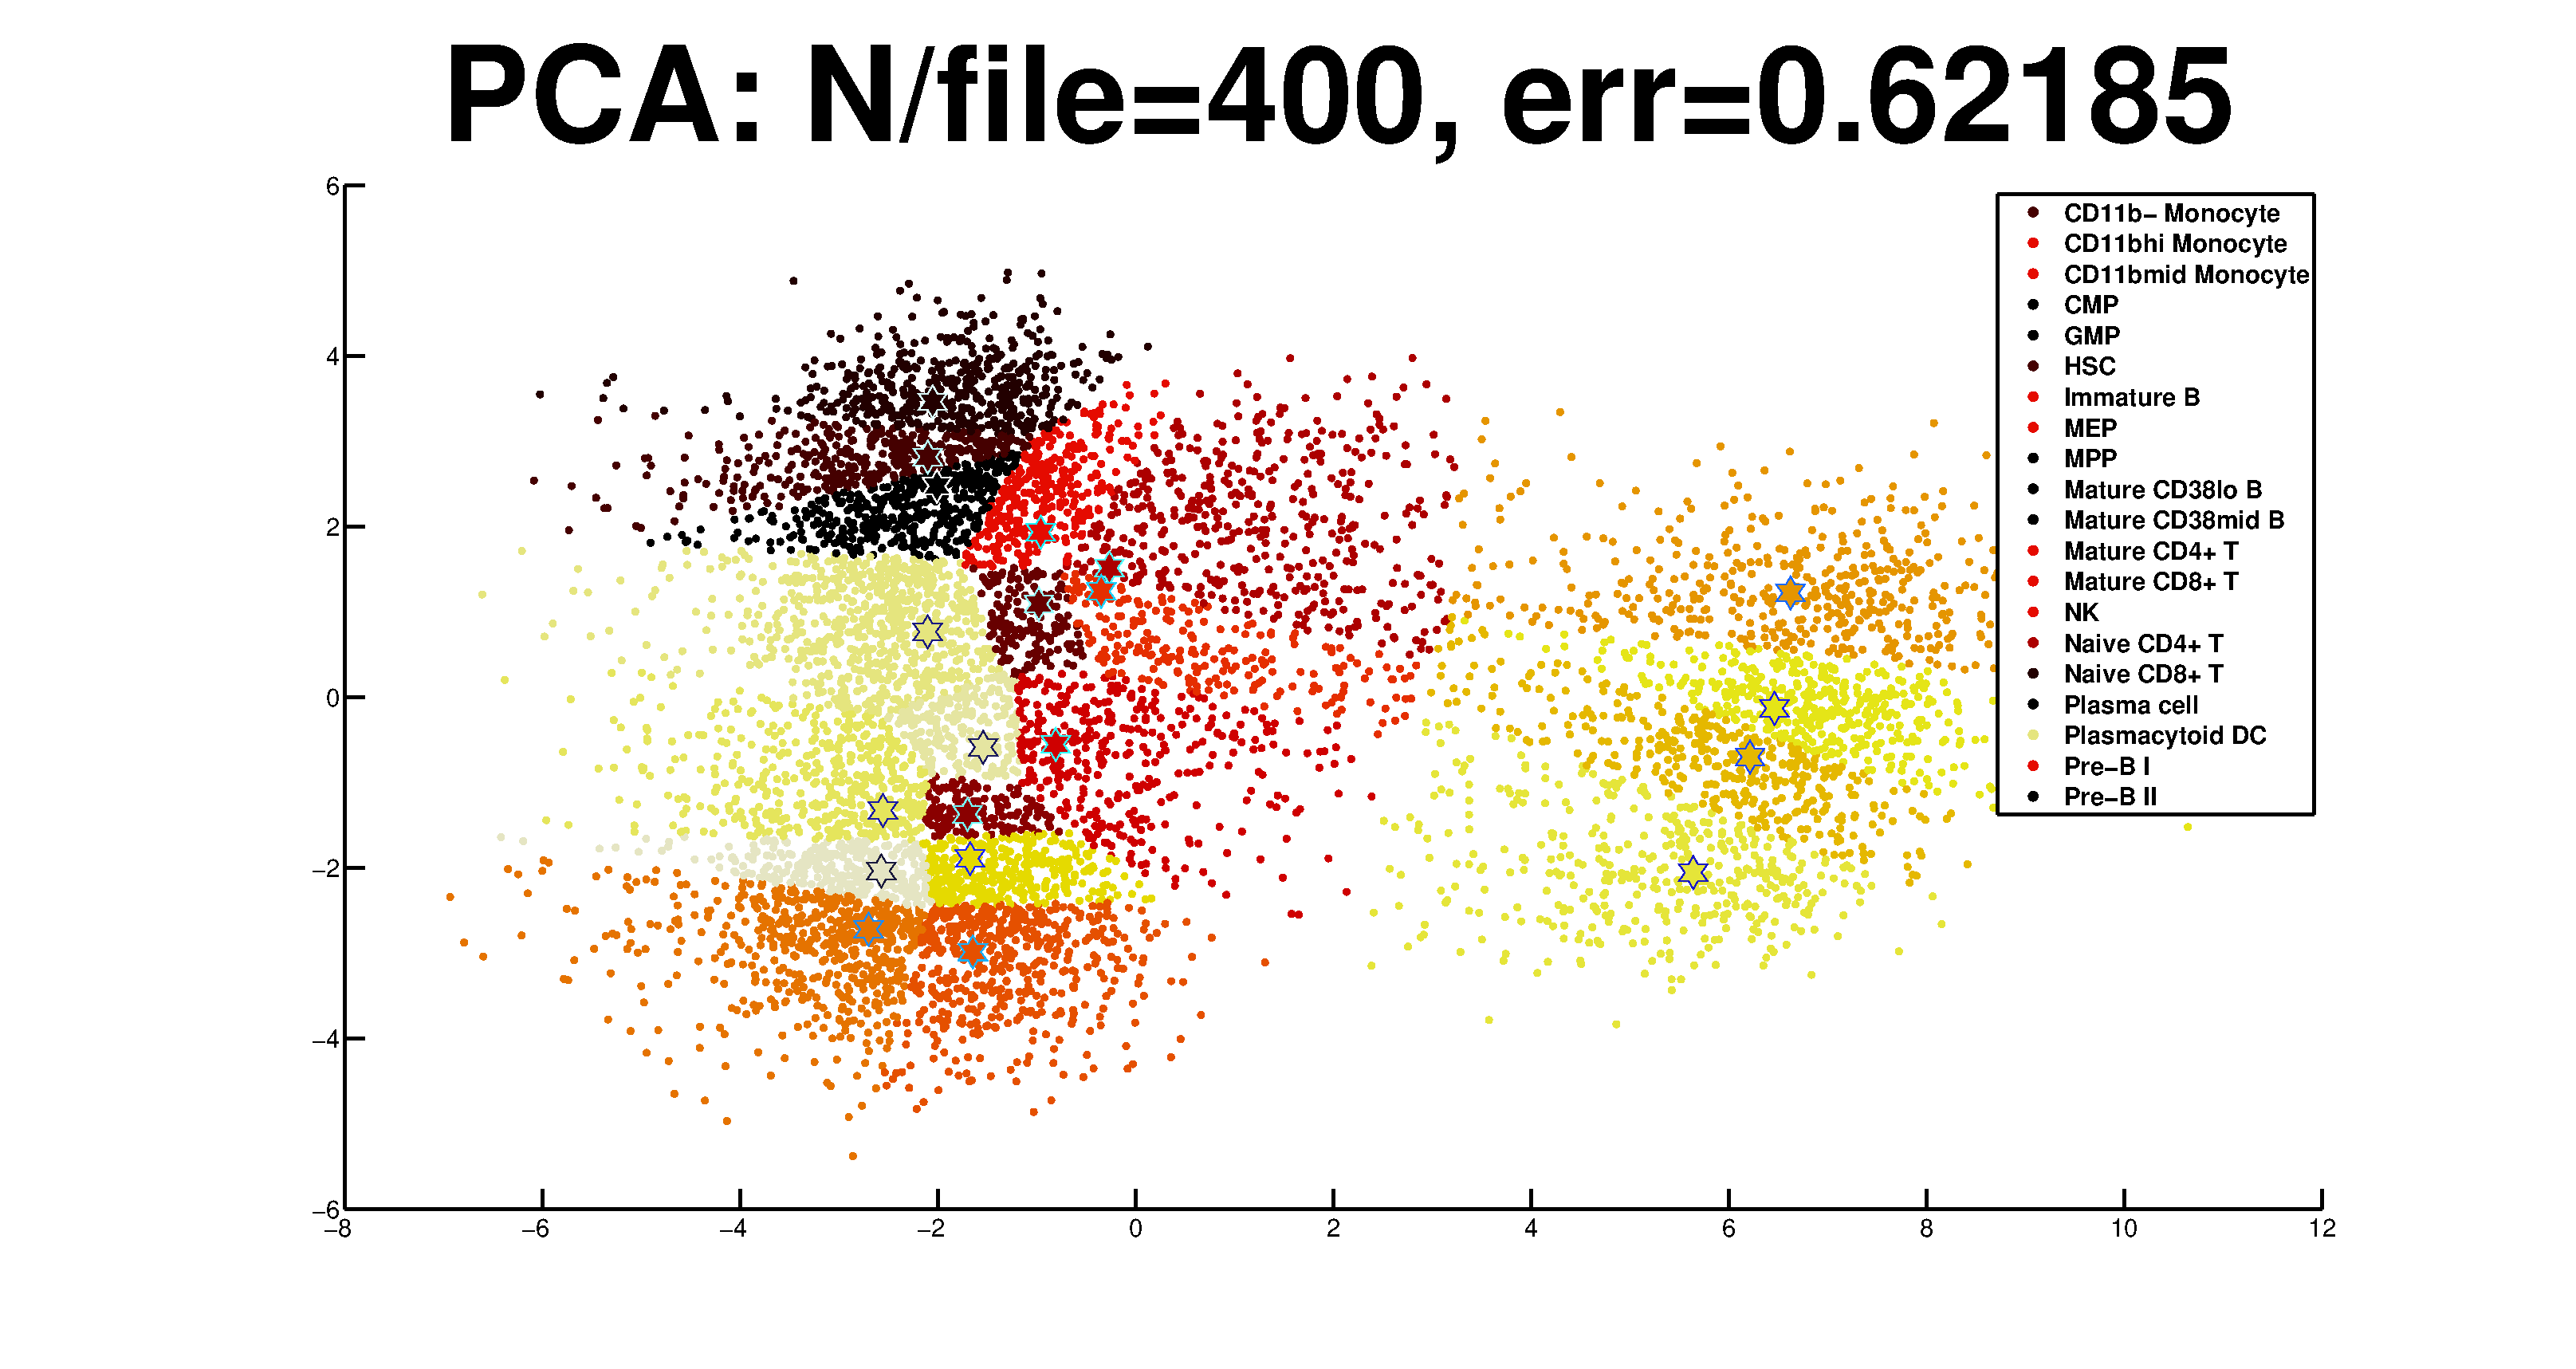
\includegraphics[width=0.47 \columnwidth,  trim = 2.5in 0.5in 1in 2in]{PCA_AllCells_N=400_relabel}}\quad
\end{center}
\caption{Principal Components Analysis on all cell sub-types with 400 cells per subtype}
\label{pca_plots_allcells}
\vskip 0.2in
\end{figure}

Even when we reduce the number of sub-types to 7 (Monocytes and T cells), the performance is still abysmal at 48.43\% error, as shown in Figure ~\ref{pca_plots_monocytes&T}.

\begin{figure}[h]
\vskip 0.2in
%\centering
\begin{center}
\subfloat[Original Labels]{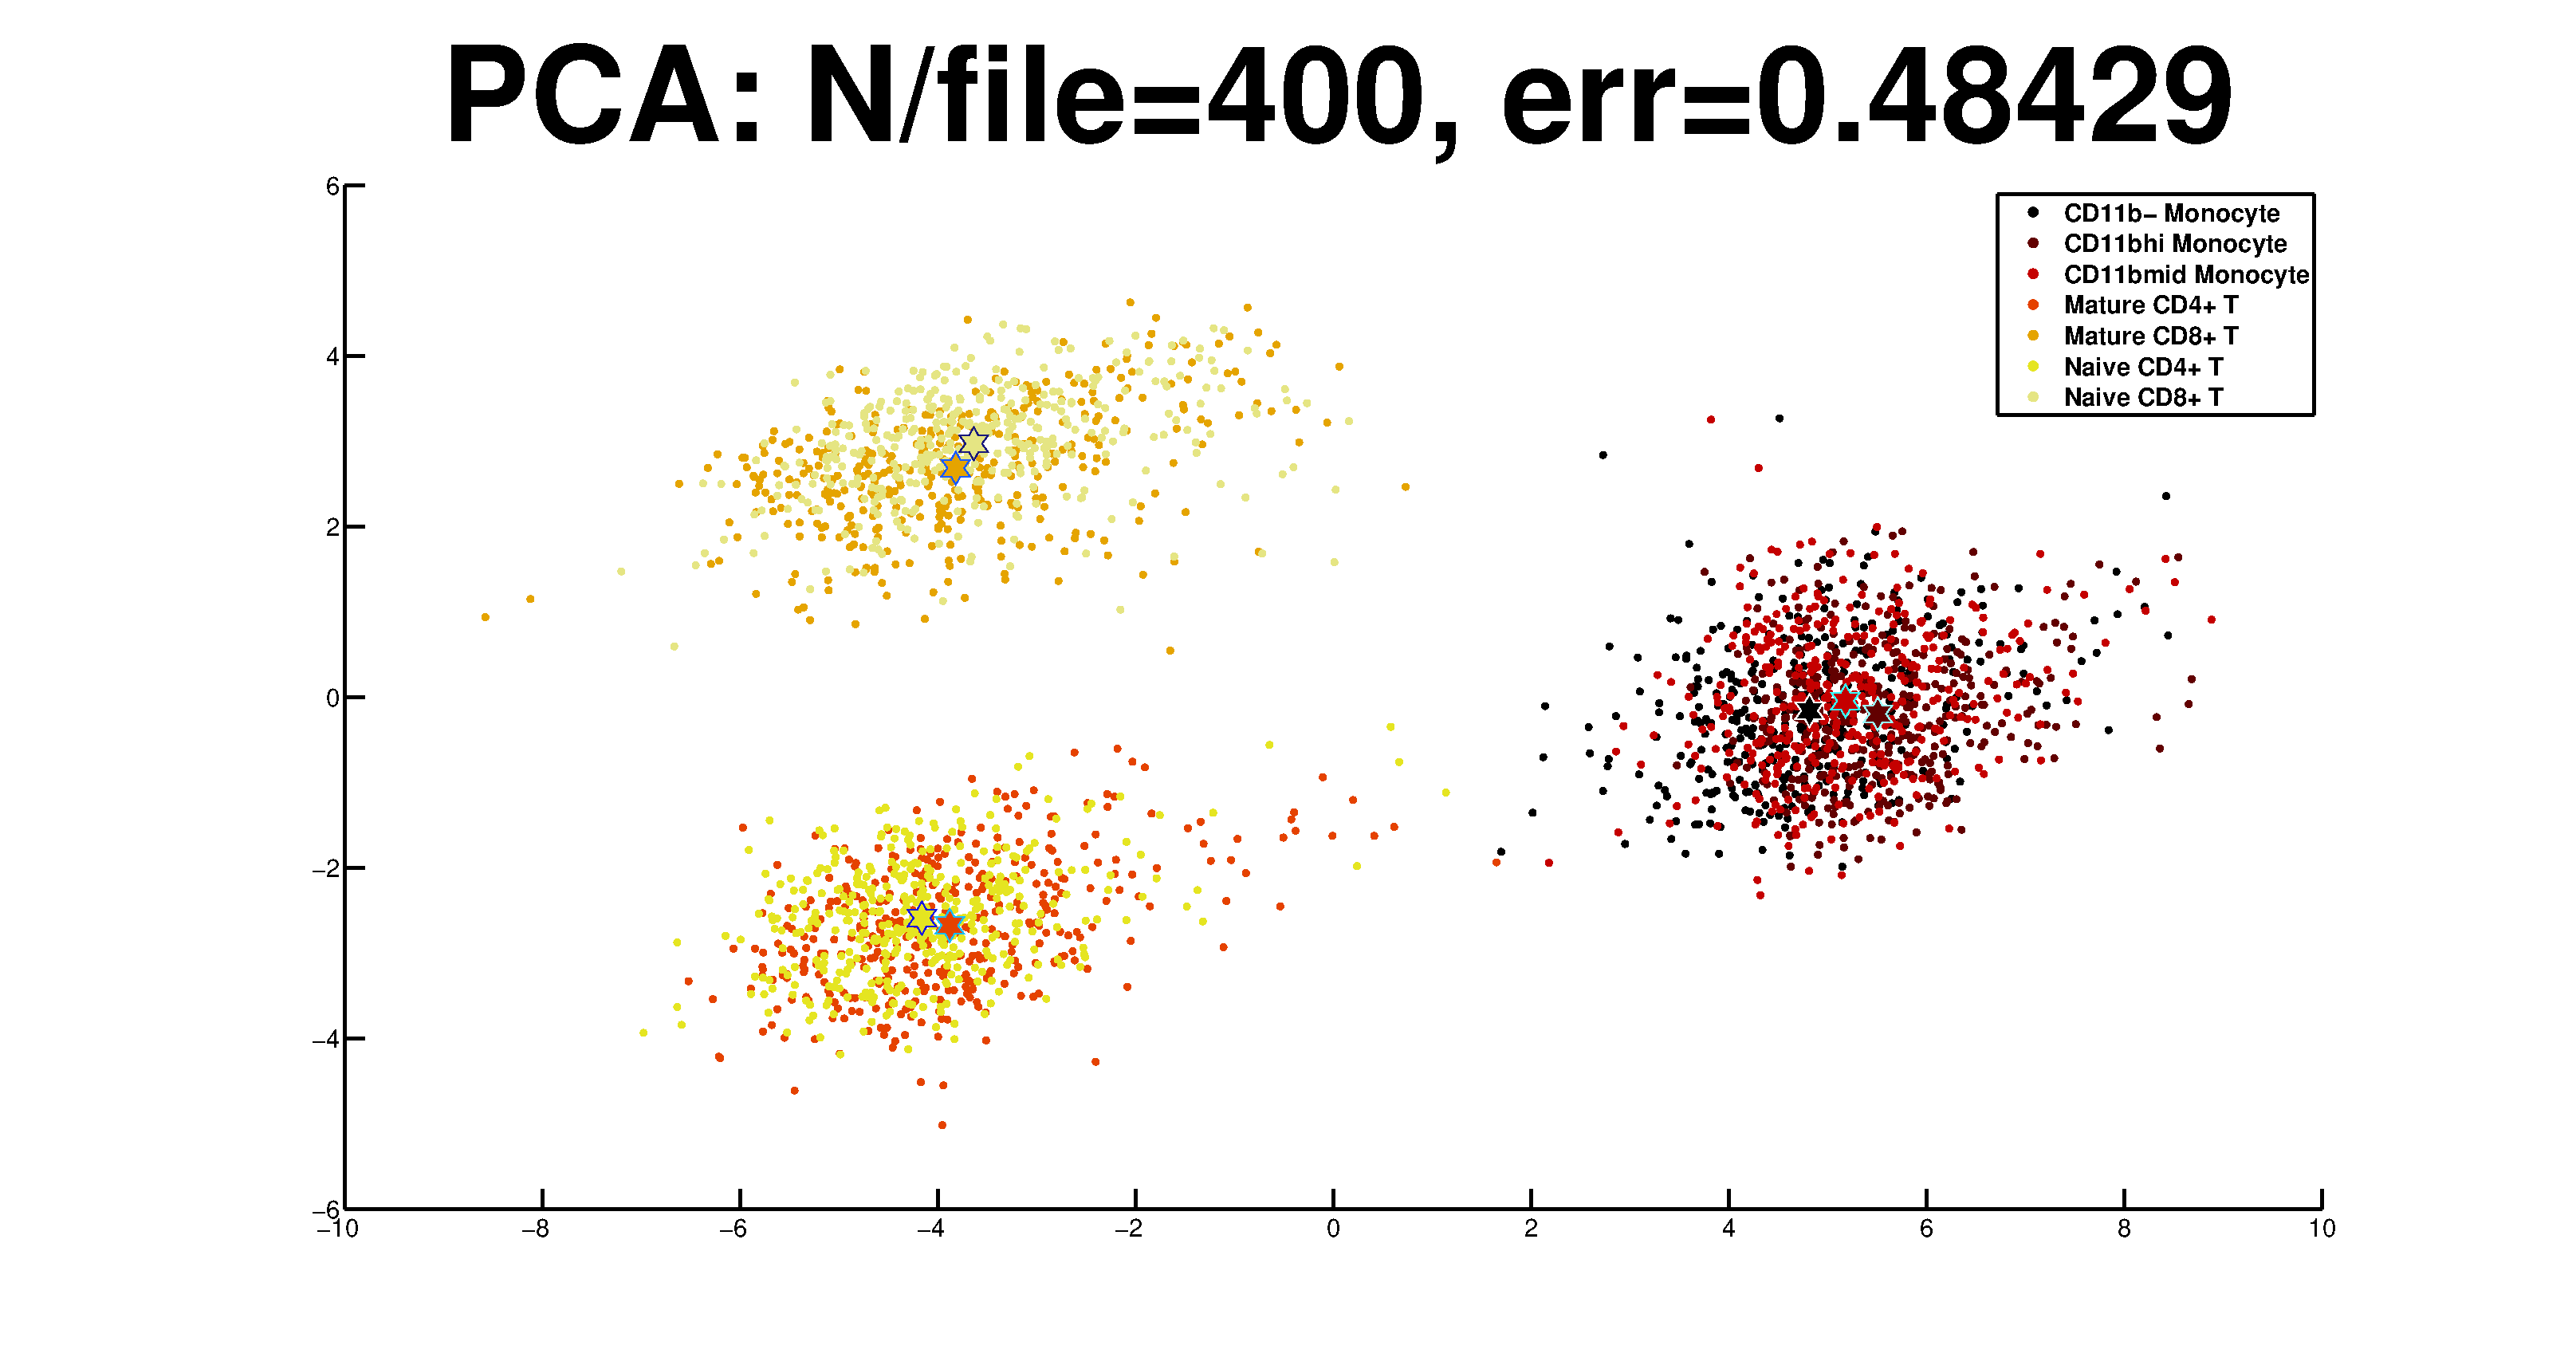
\includegraphics[width=0.47\columnwidth, trim = 2.5in 0.5in 1in 2in]{PCA_T&Moncytes_N=400}}\quad
\subfloat[New Labels]{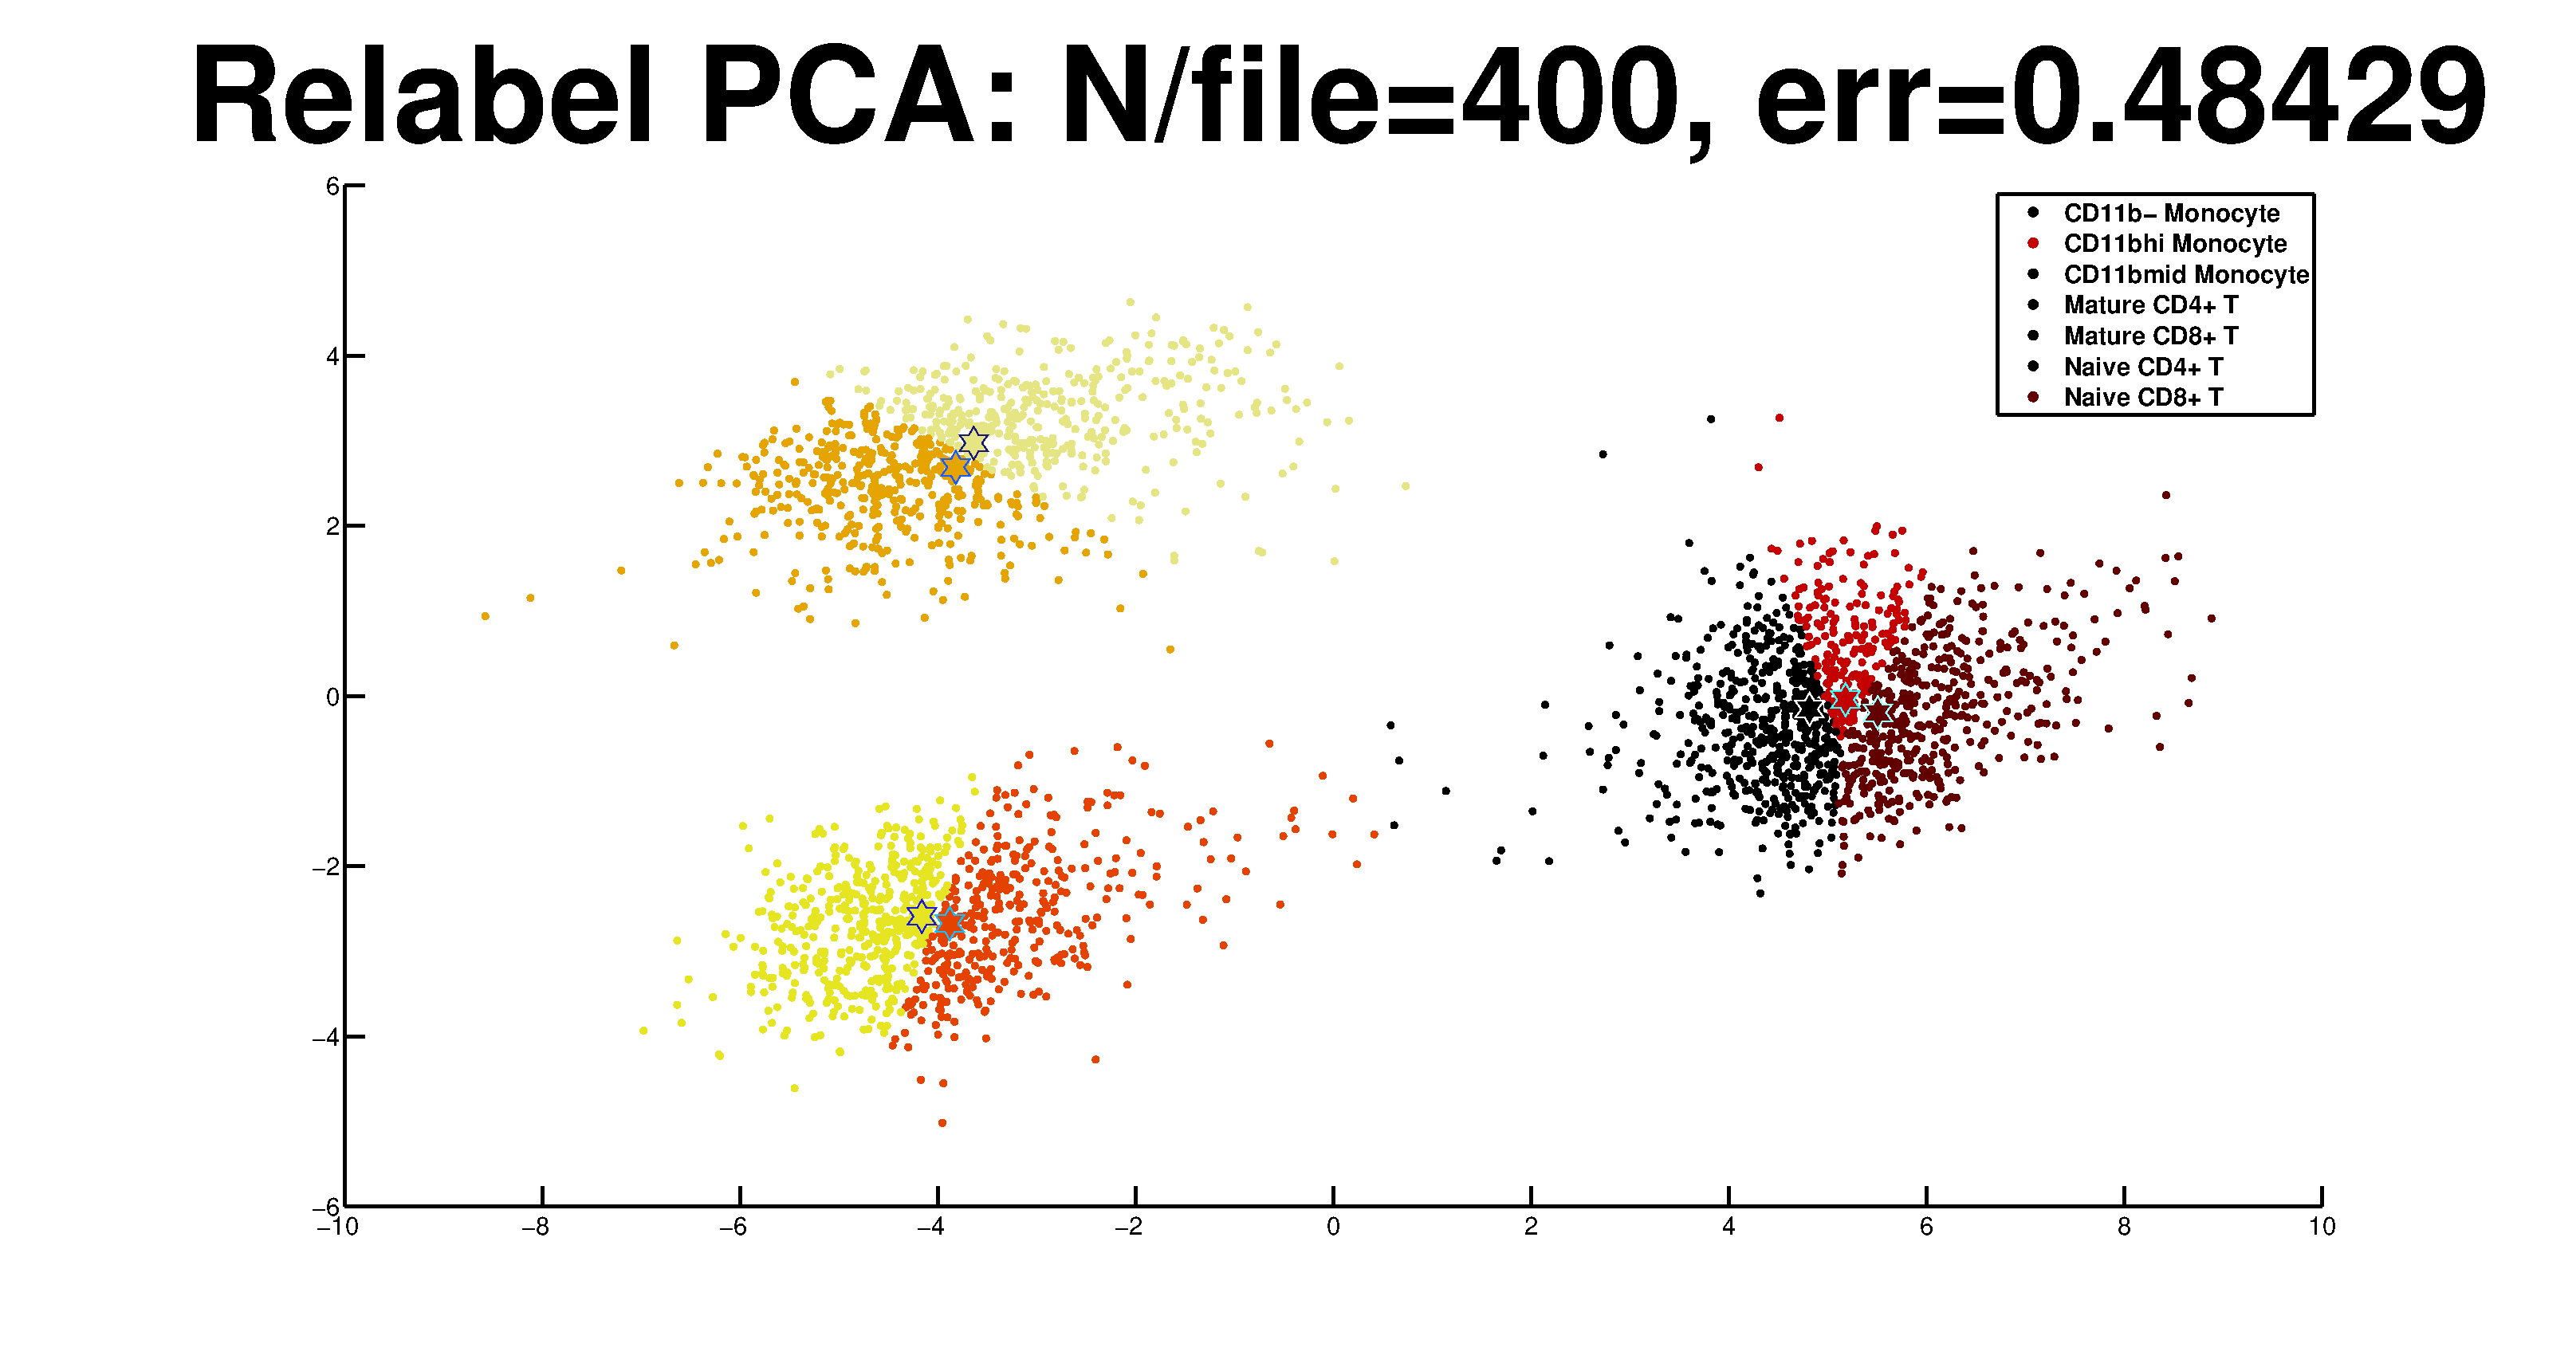
\includegraphics[width=0.47 \columnwidth,  trim = 2.5in 0.5in 1in 2in]{PCA_T&Moncytes_N=400_relabel}}\quad
\end{center}
\caption{Principal Components Analysis on Monocytes and T Cells with 400 cells per subtype}
\label{pca_plots_monocytes&T}
\vskip -0.2in
\end{figure}

\subsection{Spectral Methods - ISOMAP}
We illustrate in Figure~\ref{isomaps} the spectral method ISOMAP on this data both for all cell sub-types (N/type = 100) and for just monocytes and T cells (N/type = 400) combined. In each case, the algorithm yields no discernible segmented high-level structure.

\begin{figure}[h]
\vskip 0.2in
%\centering
\begin{center}
\subfloat[All cell types]{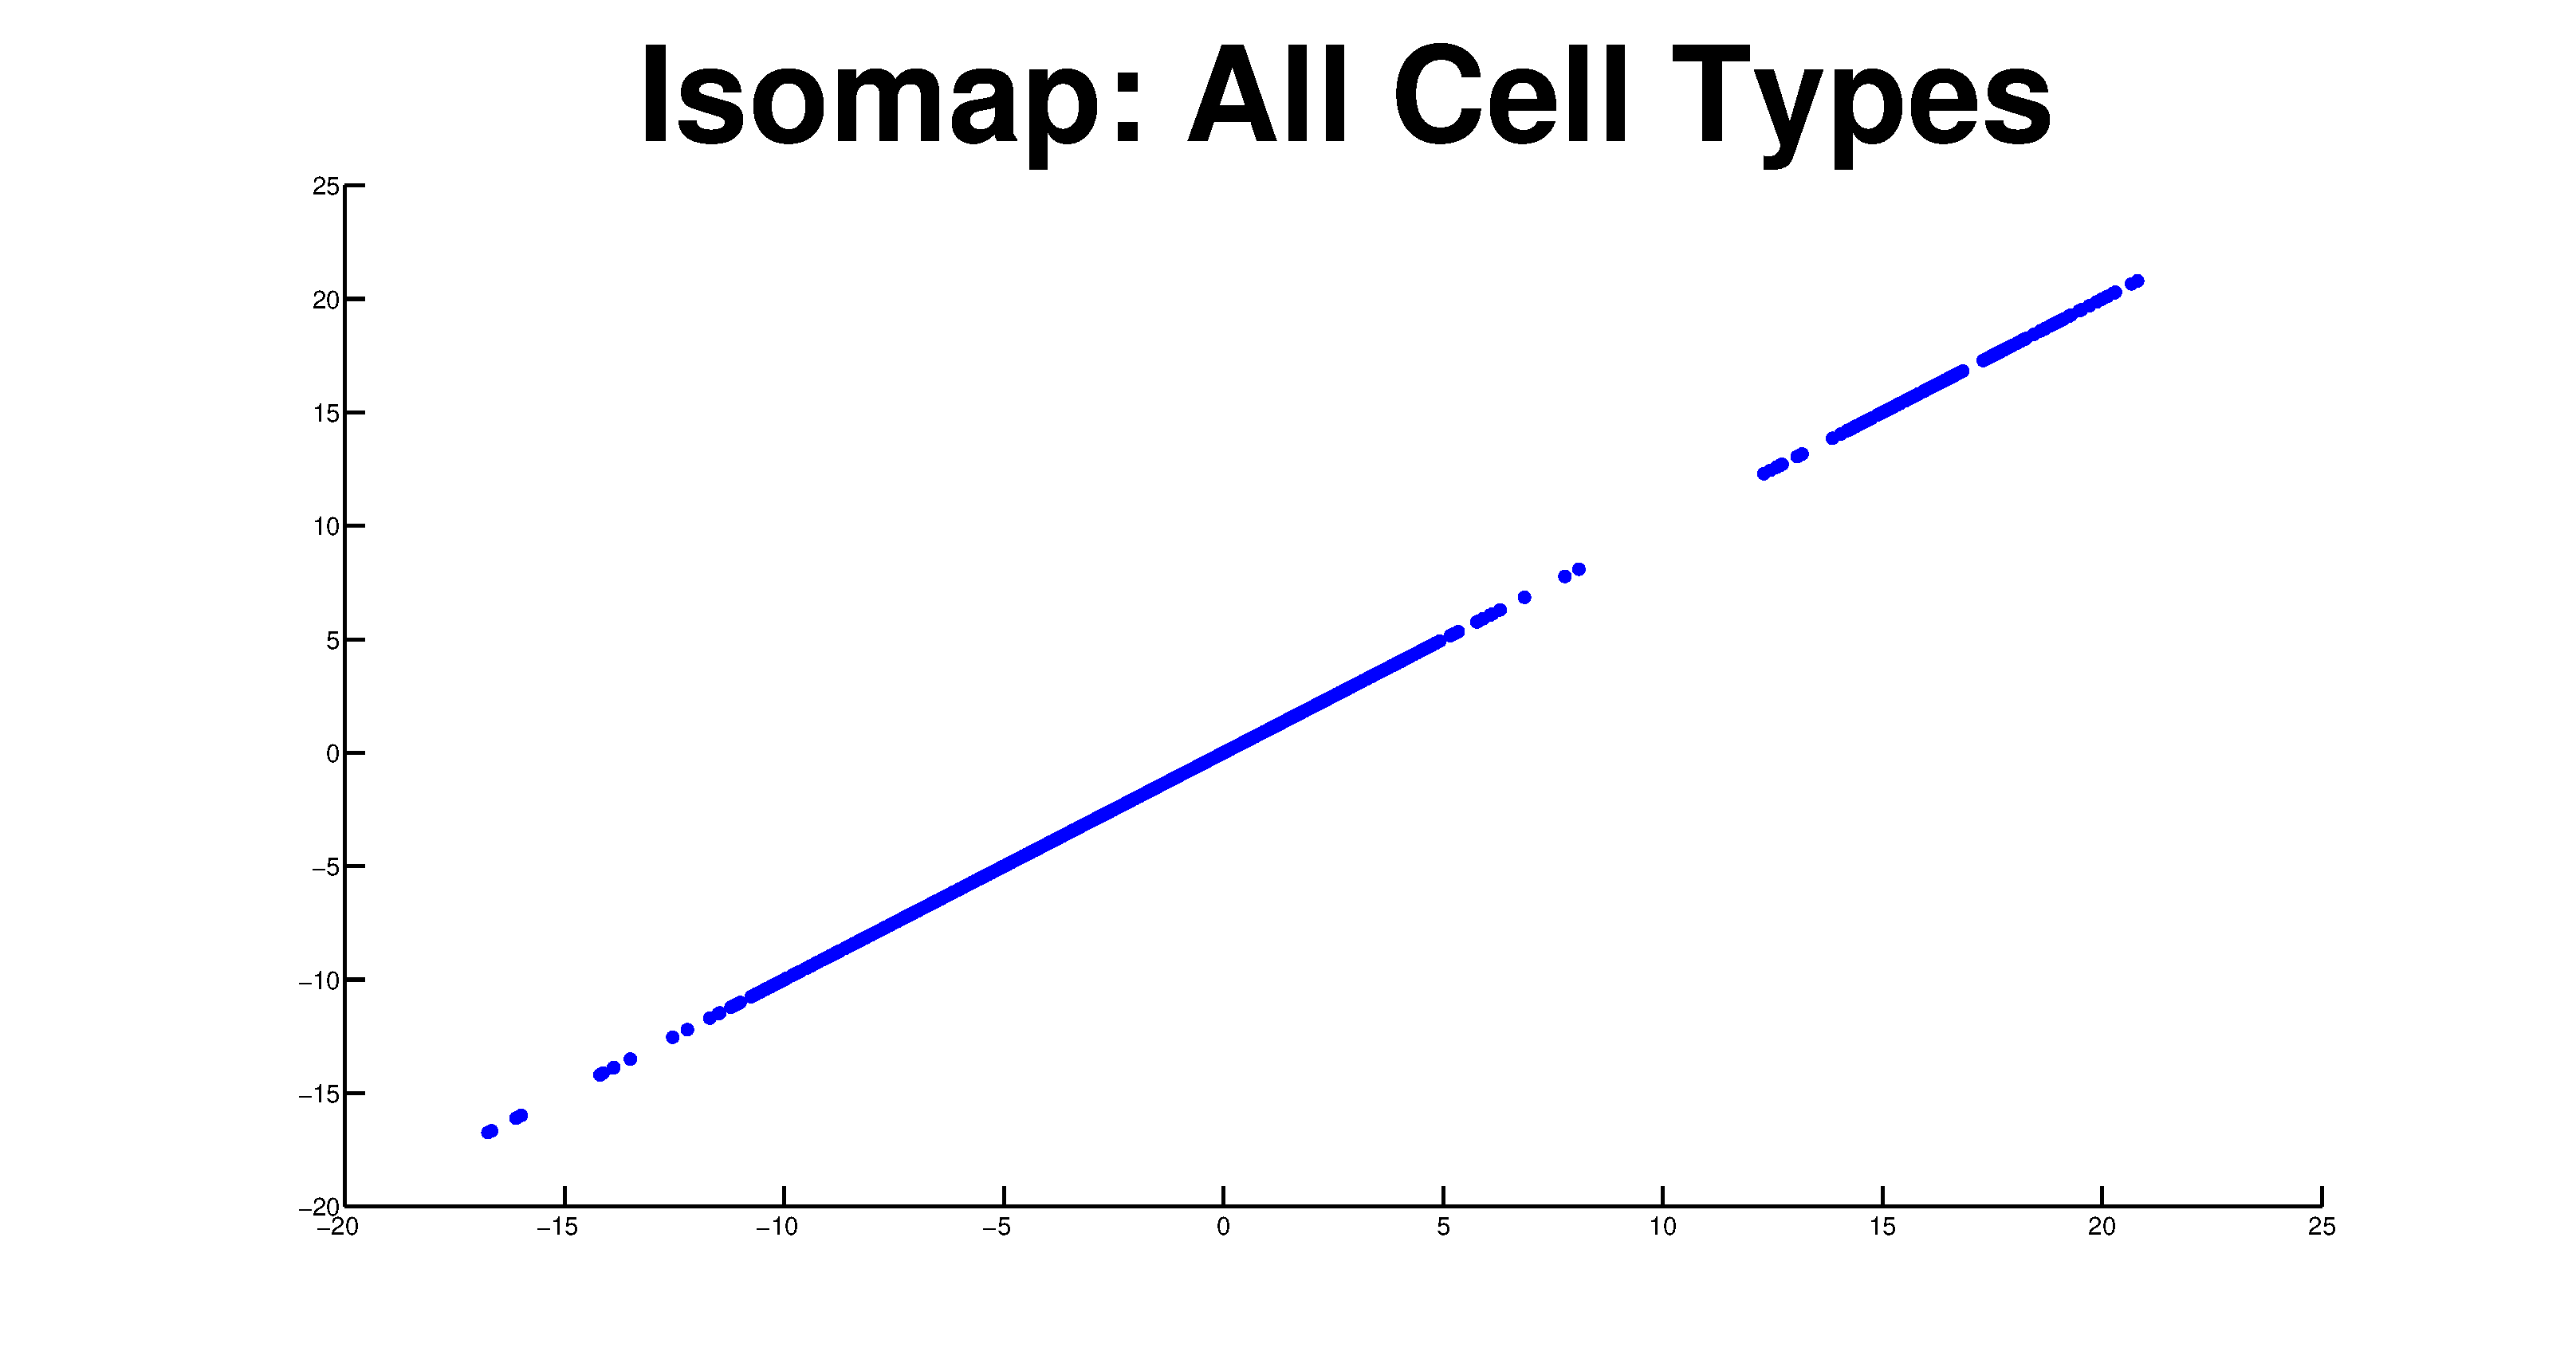
\includegraphics[width=0.47\columnwidth, trim = 2.5in 0.5in 1in 2in]{ISOMAP_AllCells_N=100}}\quad
\subfloat[Monocytes and T Cells]{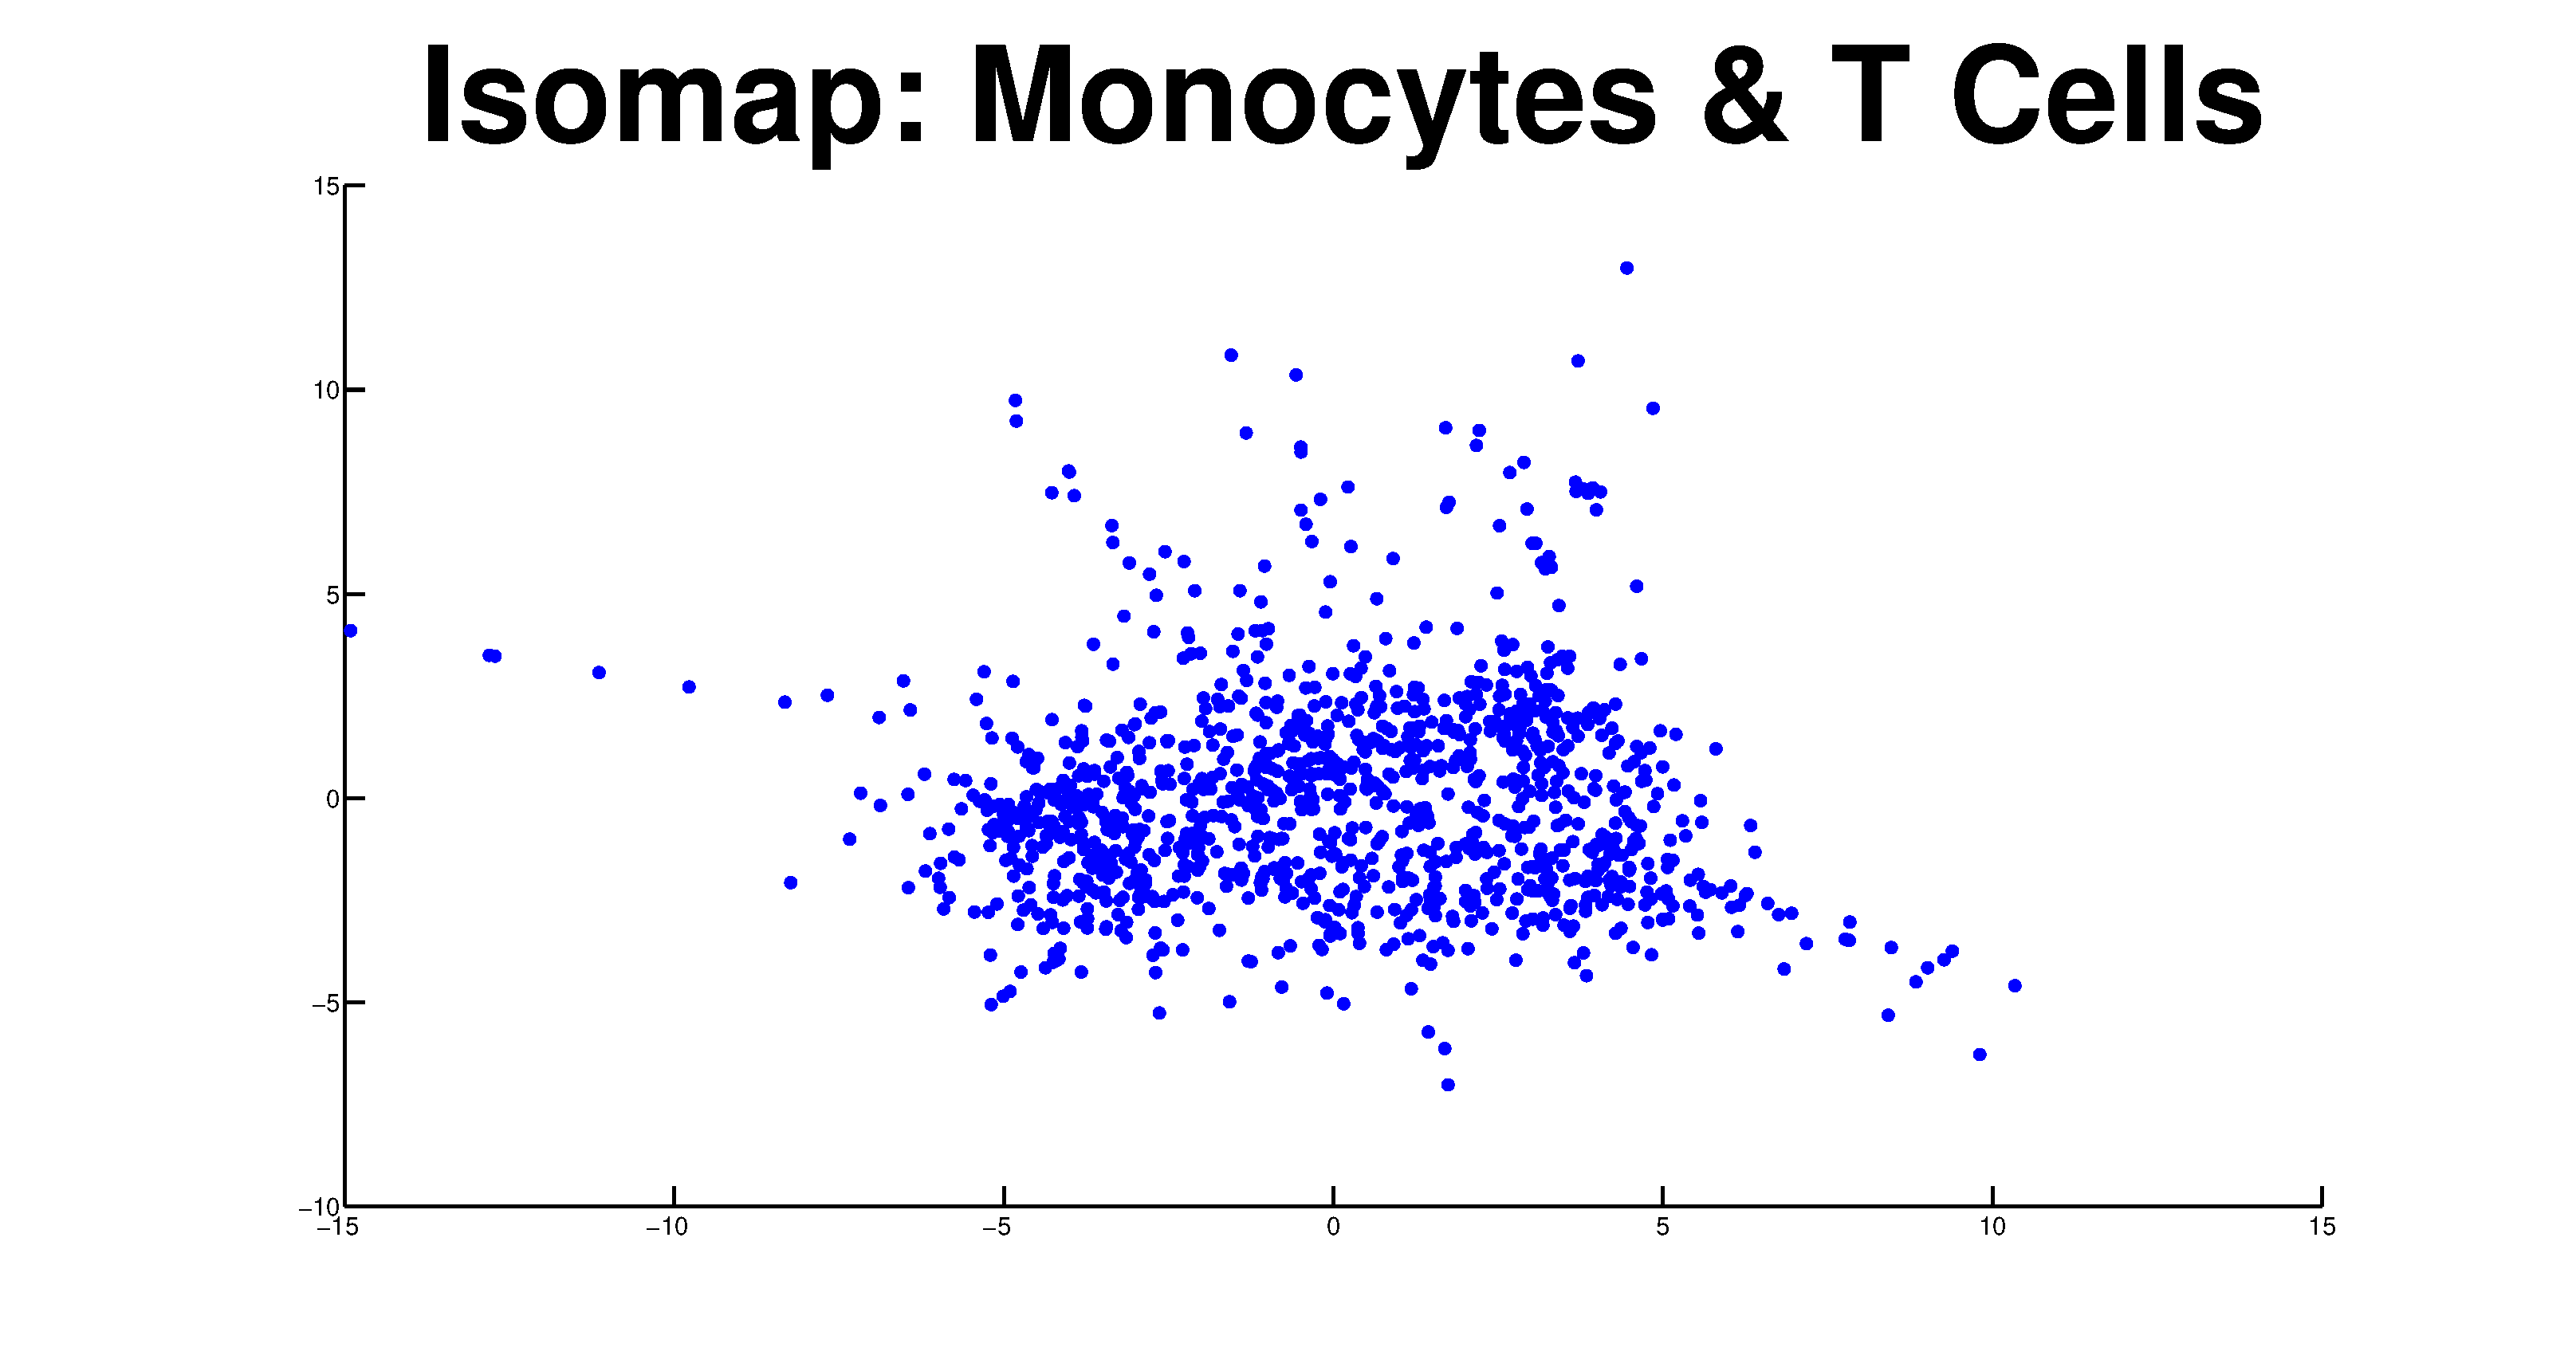
\includegraphics[width=0.47 \columnwidth,  trim = 2.5in 0.5in 1in 2in]{ISOMAP_Monoctypes&TCells_N=400}}\quad
\end{center}
\caption{ISOMAP with 400 cells per subtype}
\label{isomaps}
\vskip -0.2in
\end{figure}

\subsection{Nonlinear Methods}
We begin by considering t-SNE and sampling 400 cells from each cell type. We see in Figure~\ref{tSNEall} that the algorithm clusters the points reasonably well, even though it attains a relatively high error of 24.33\%. On the other hand, when we only work with Monocytes and T Cells (Figure~\ref{tSNEmonocytesandtcells}), we obtain a 7.46\% error - a 7-fold improvement on PCA for the same data set. 

Next, we consider s-SNE on a similar sample of 400 cells taken from either all cell types (Figure~\ref{sSNEall})  or  Monocytes and T Cells (Figure~\ref{sSNEmonocytesandtcells}). We see that the visualization appears to perform as well as tSNE, yet the metric shows that its performance is slightly worse. sSNE attained errors of 28.57\% and 8.18\% for all cell types and the subset of Monocytes and T Cells, respectively.  

% tSNE all
\begin{figure}[h]
\vskip 0.2in
\begin{center}
\subfloat[Original Labels]{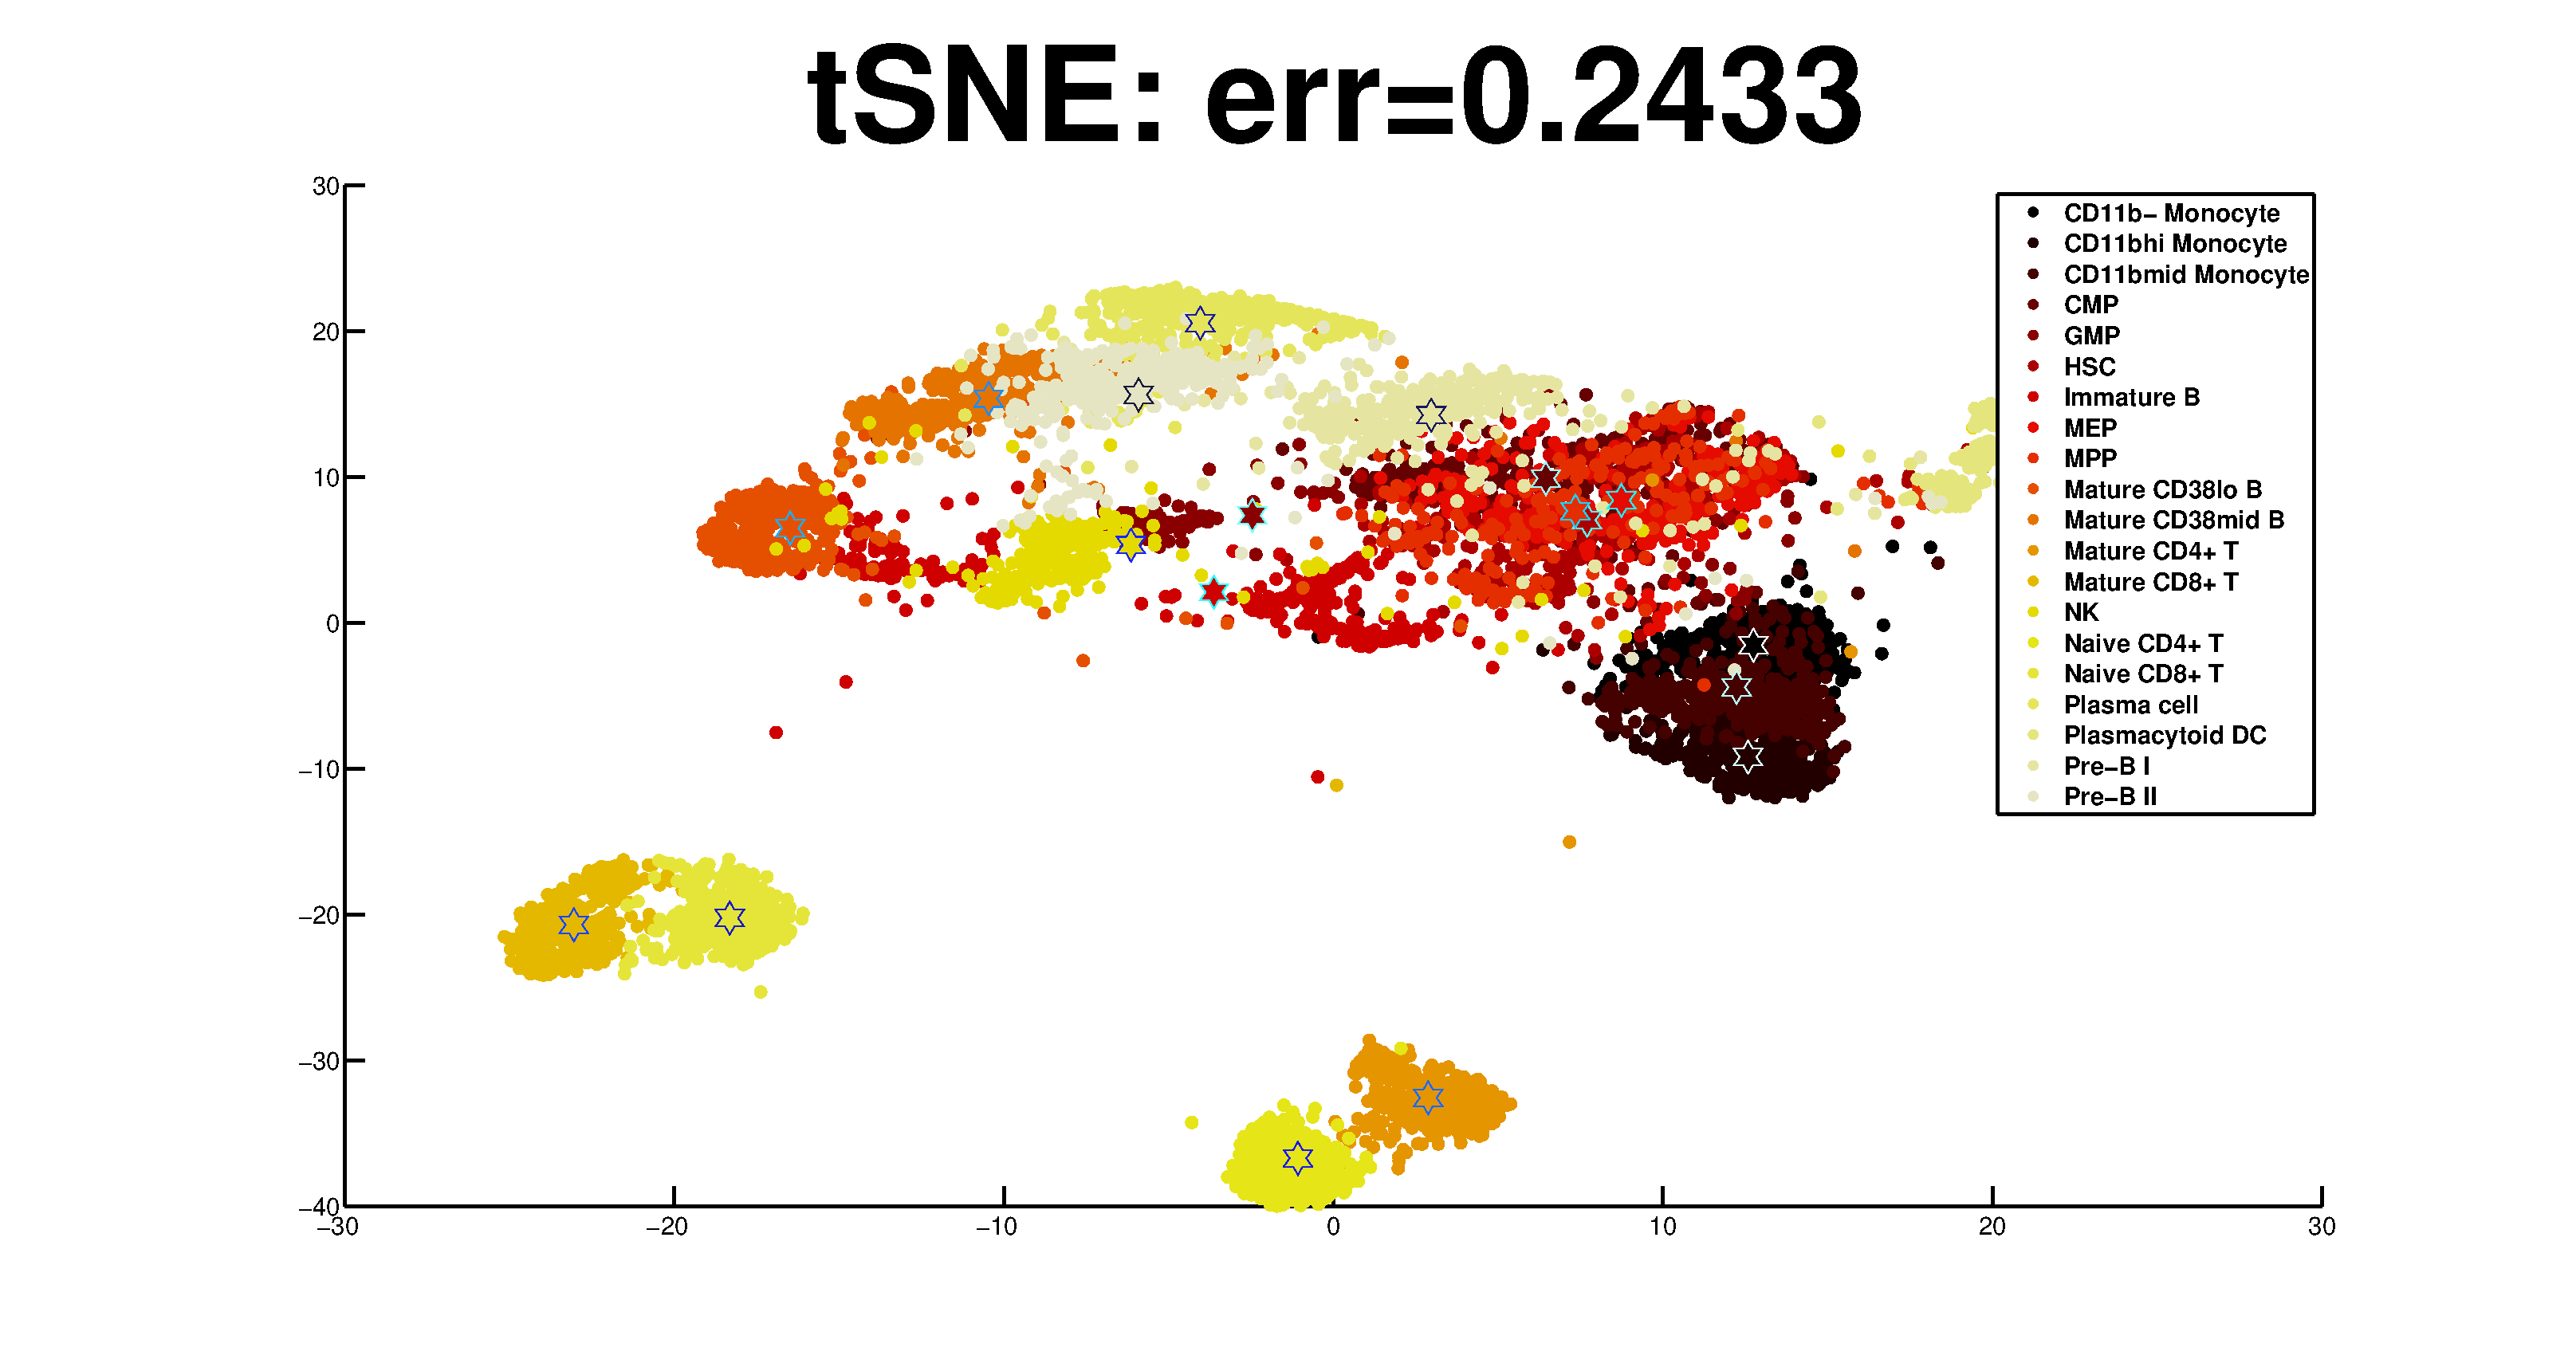
\includegraphics[width=0.47\columnwidth, trim = 2.5in 0.5in 1in 2in]{tSNE_AllCells_N=400}}\quad
\subfloat[New Labels]{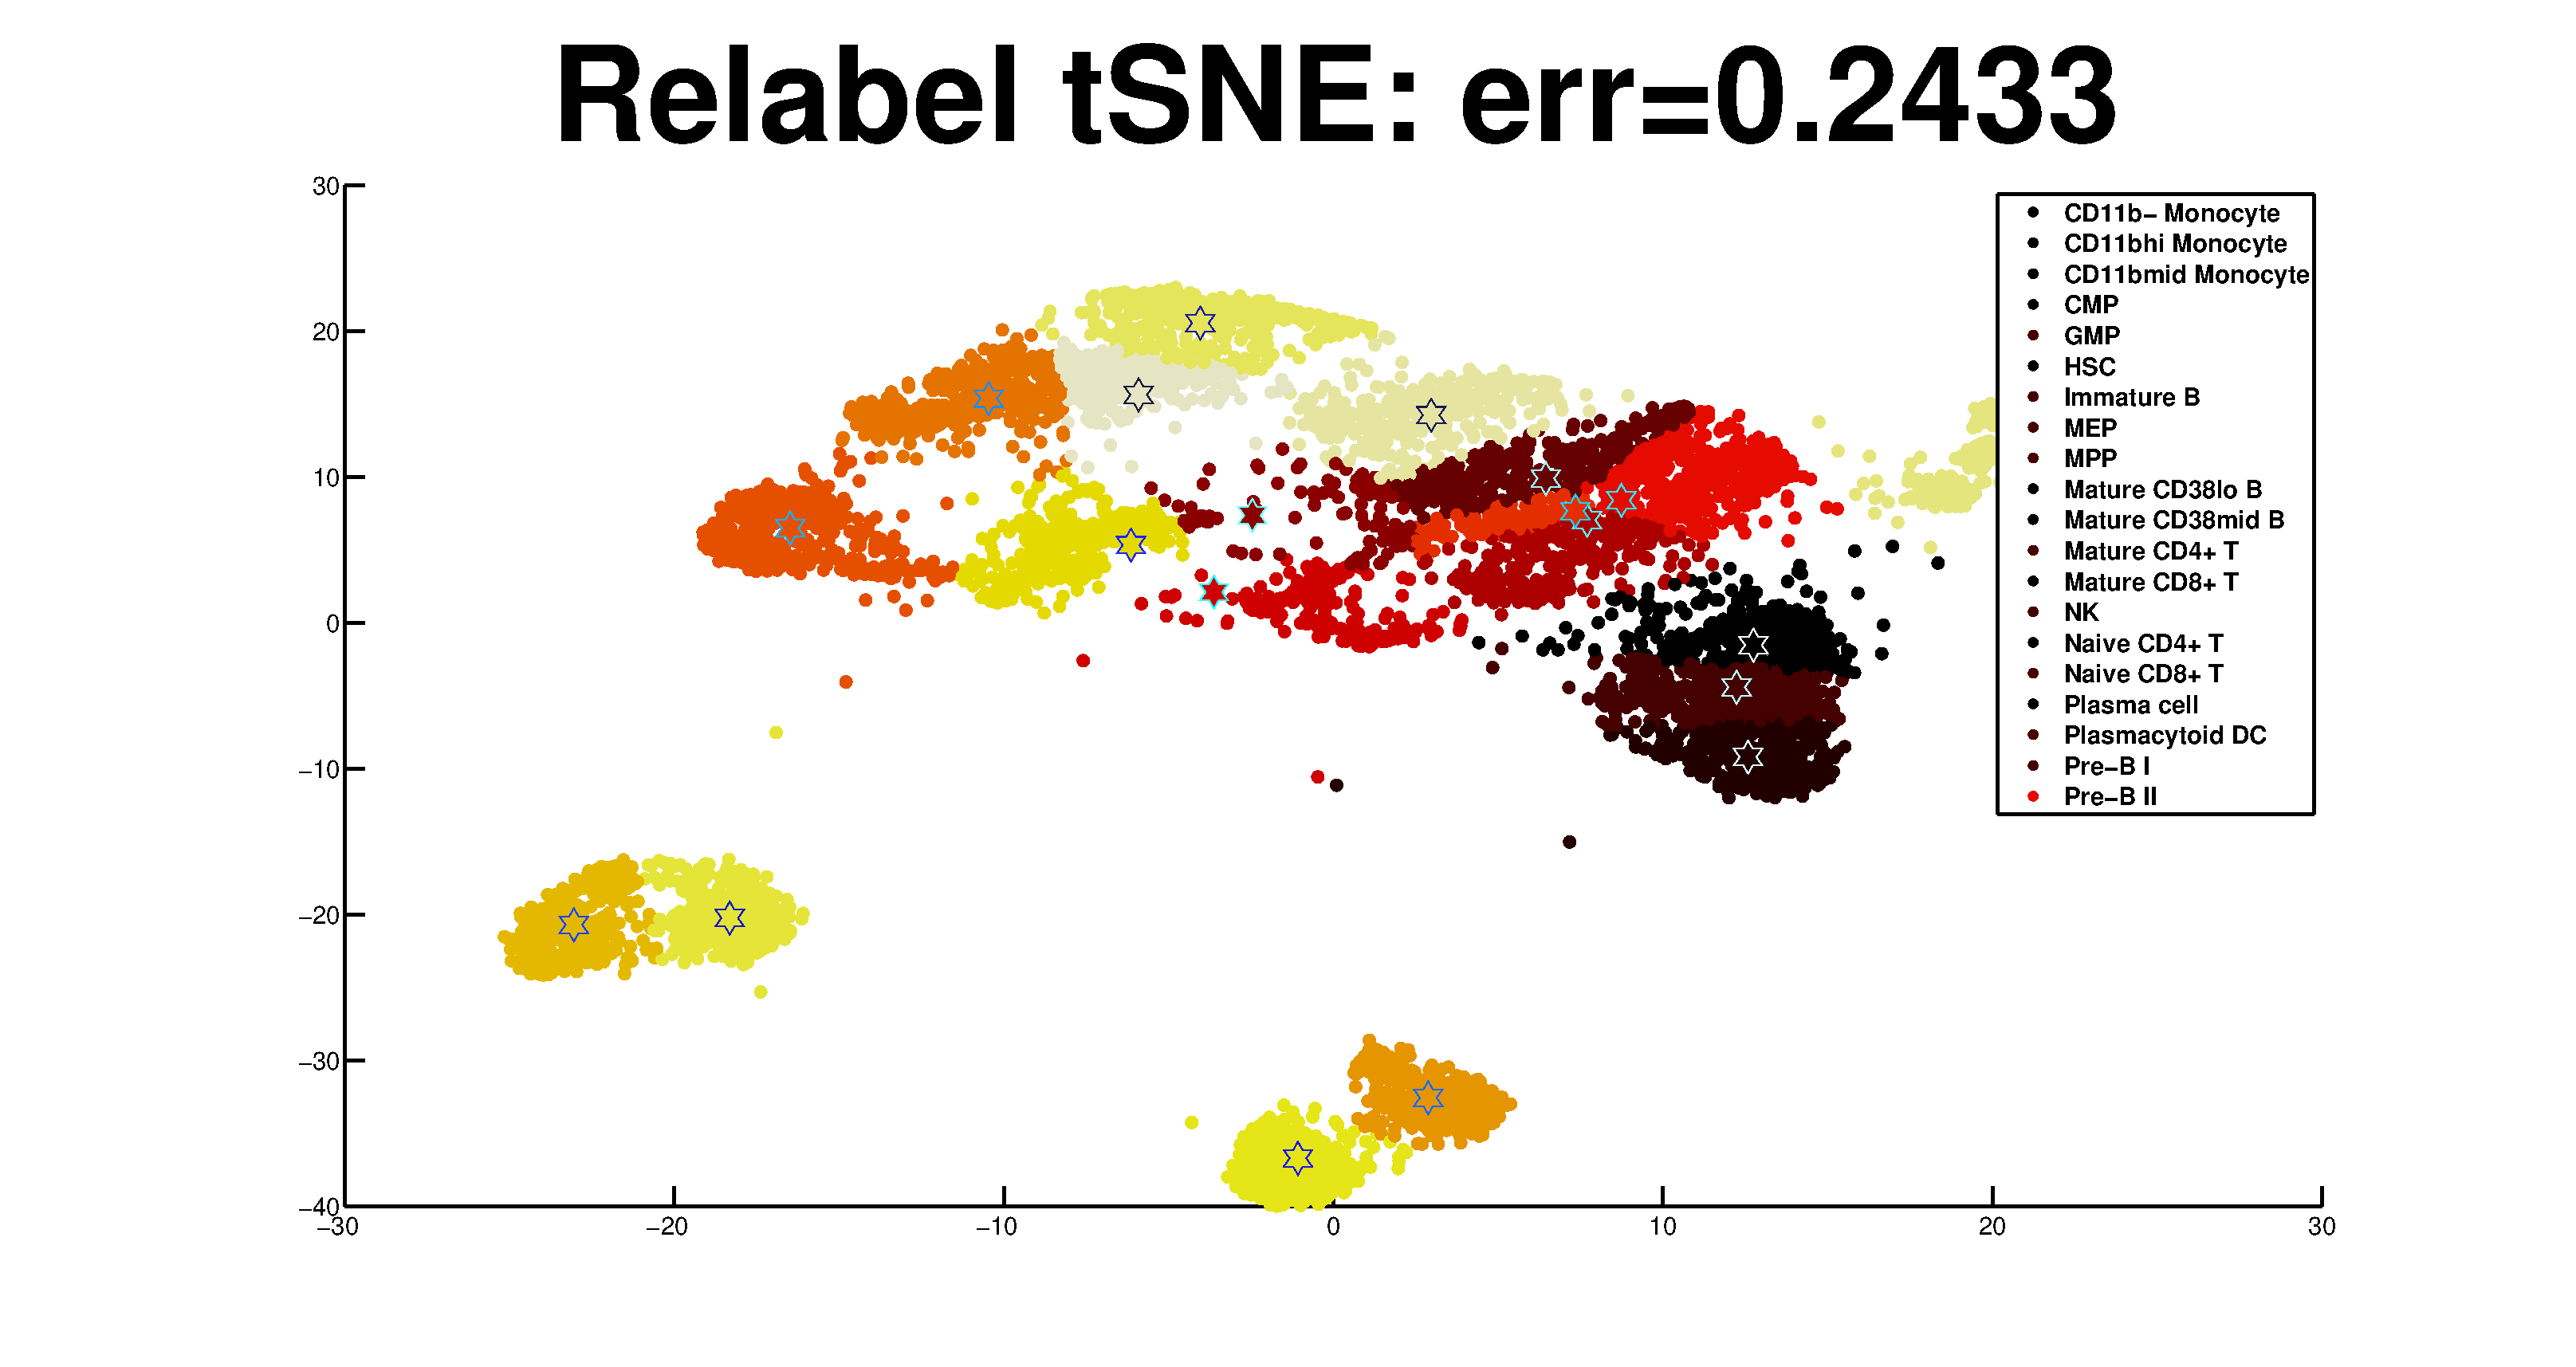
\includegraphics[width=0.47 \columnwidth,  trim = 2.5in 0.5in 1in 2in]{tSNE_AllCells_N=400_relabel}}\quad
\end{center}
\caption{tSNE on all cell sub-types with 400 cells per subtype}
\label{tSNEall}
\vskip -0.2in
\end{figure}

%tSNE monocytes and T
\begin{figure}[h]
\vskip 0.2in
\begin{center}
\subfloat[Original Labels]{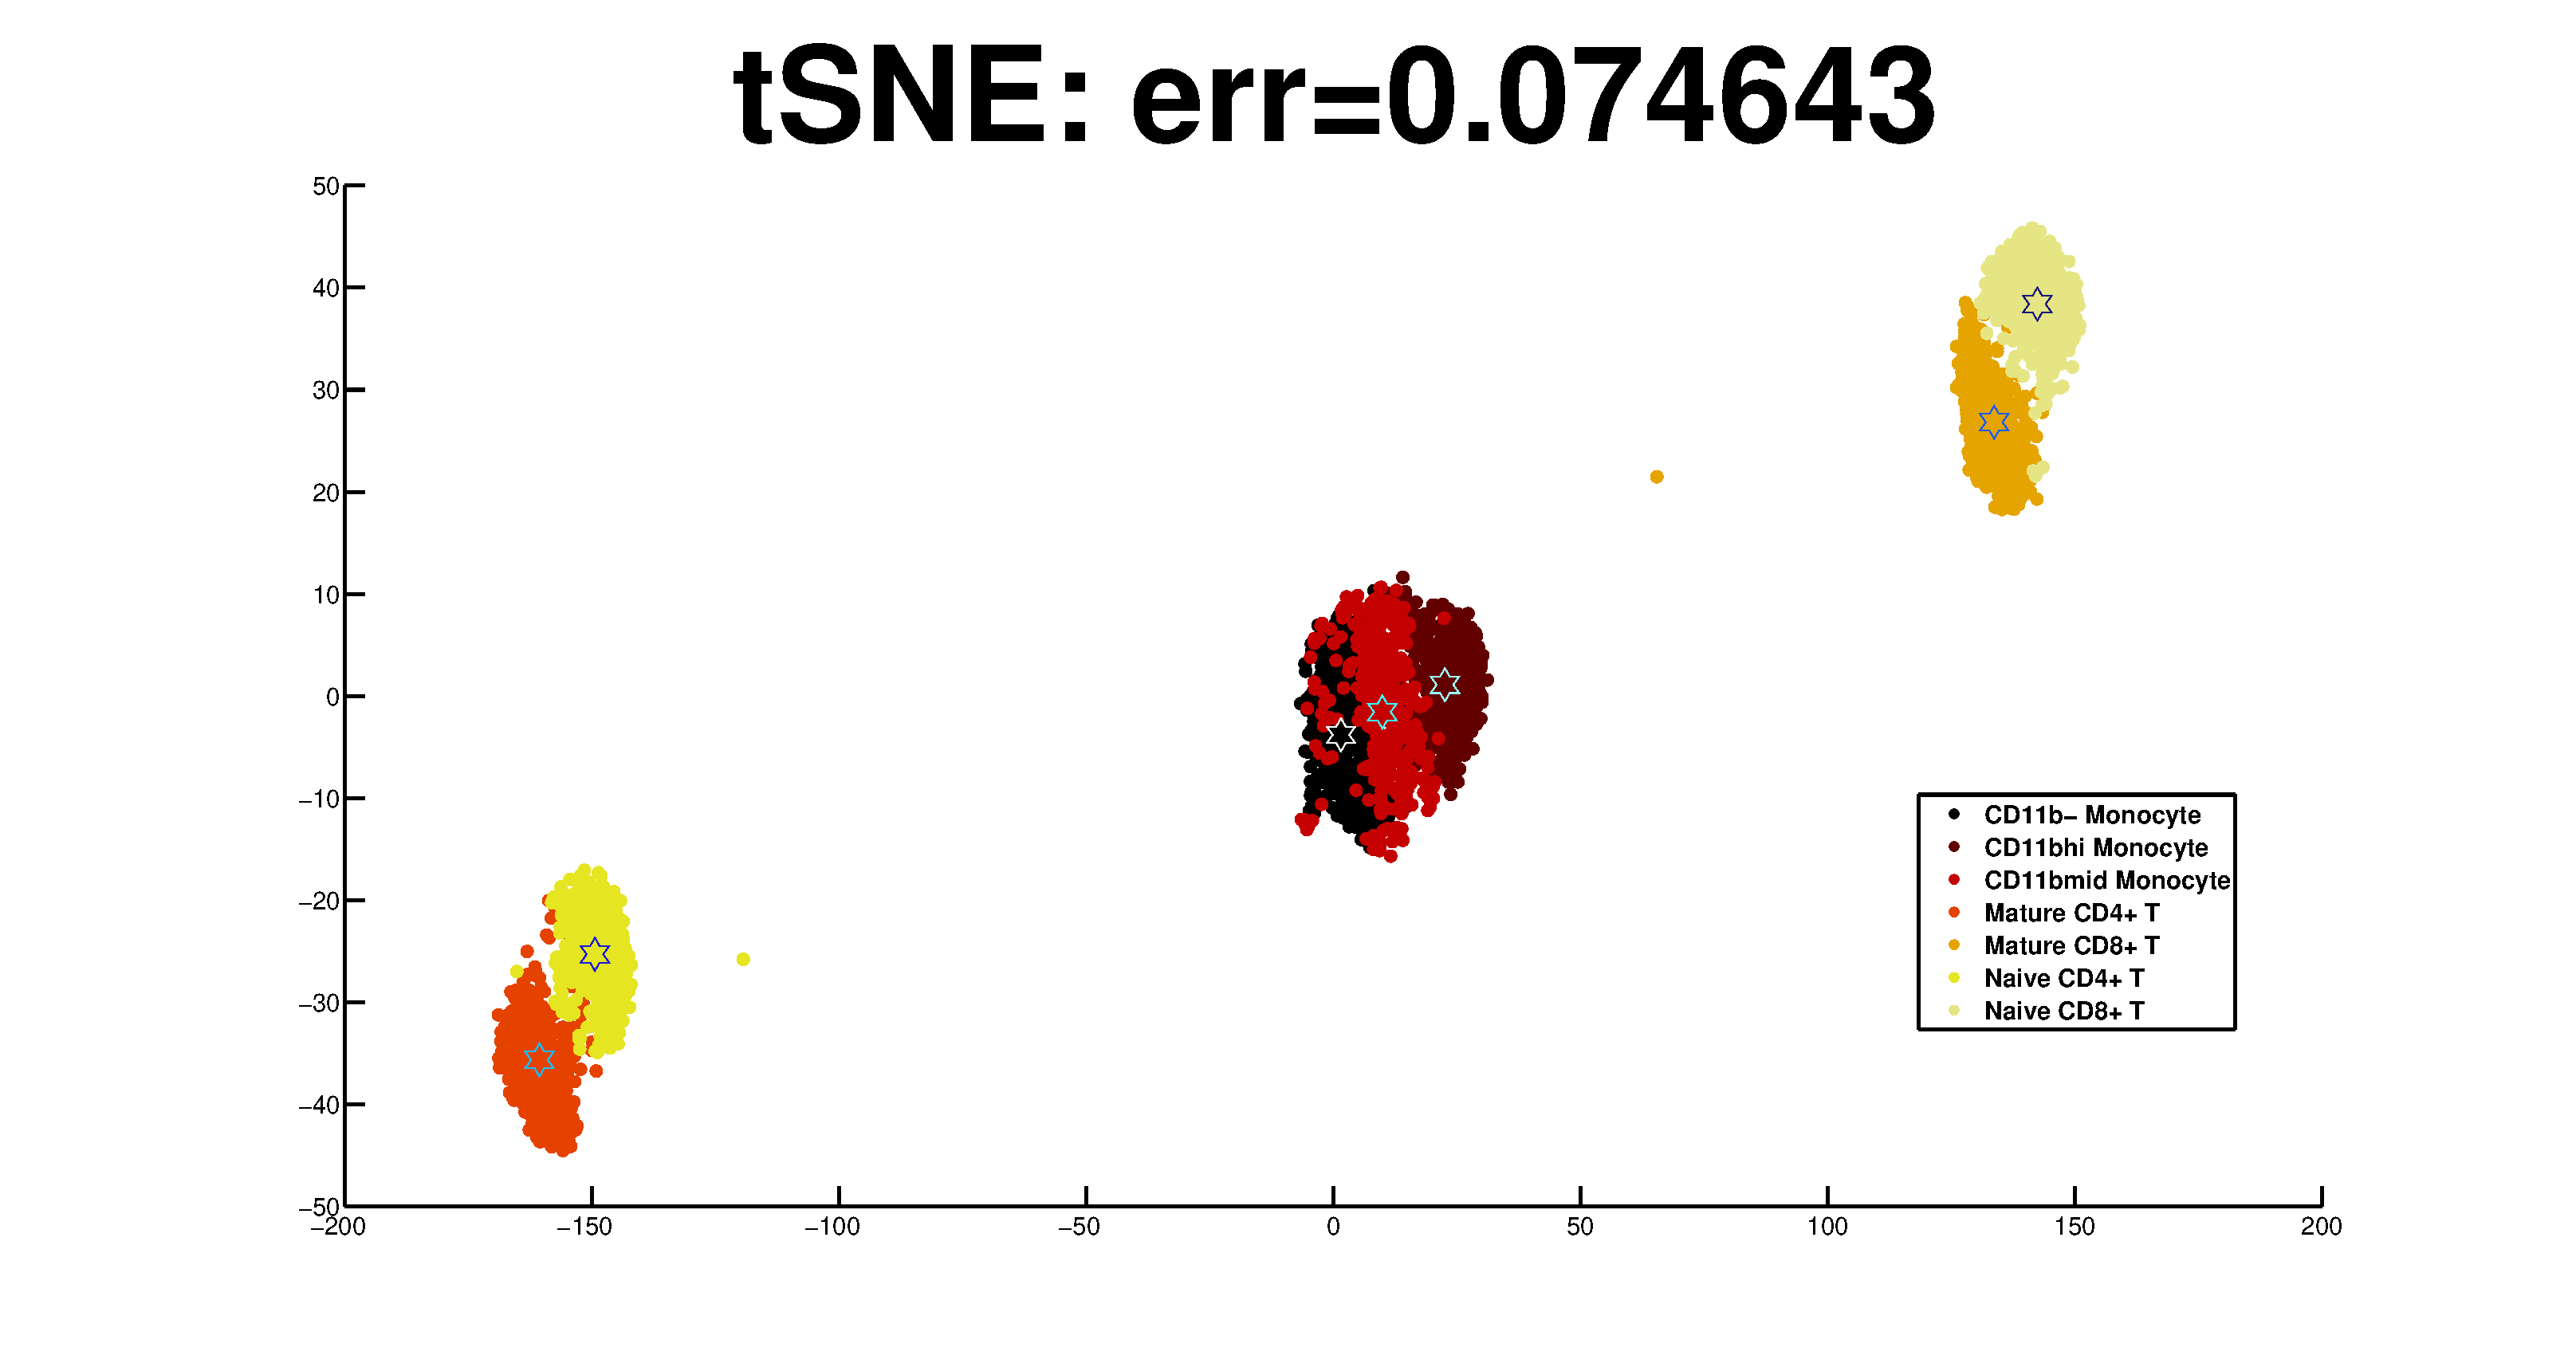
\includegraphics[width=0.47\columnwidth, trim = 2.5in 0.5in 1in 2in]{tSNE_Monocytes&TCells_N=400}}\quad
\subfloat[New Labels]{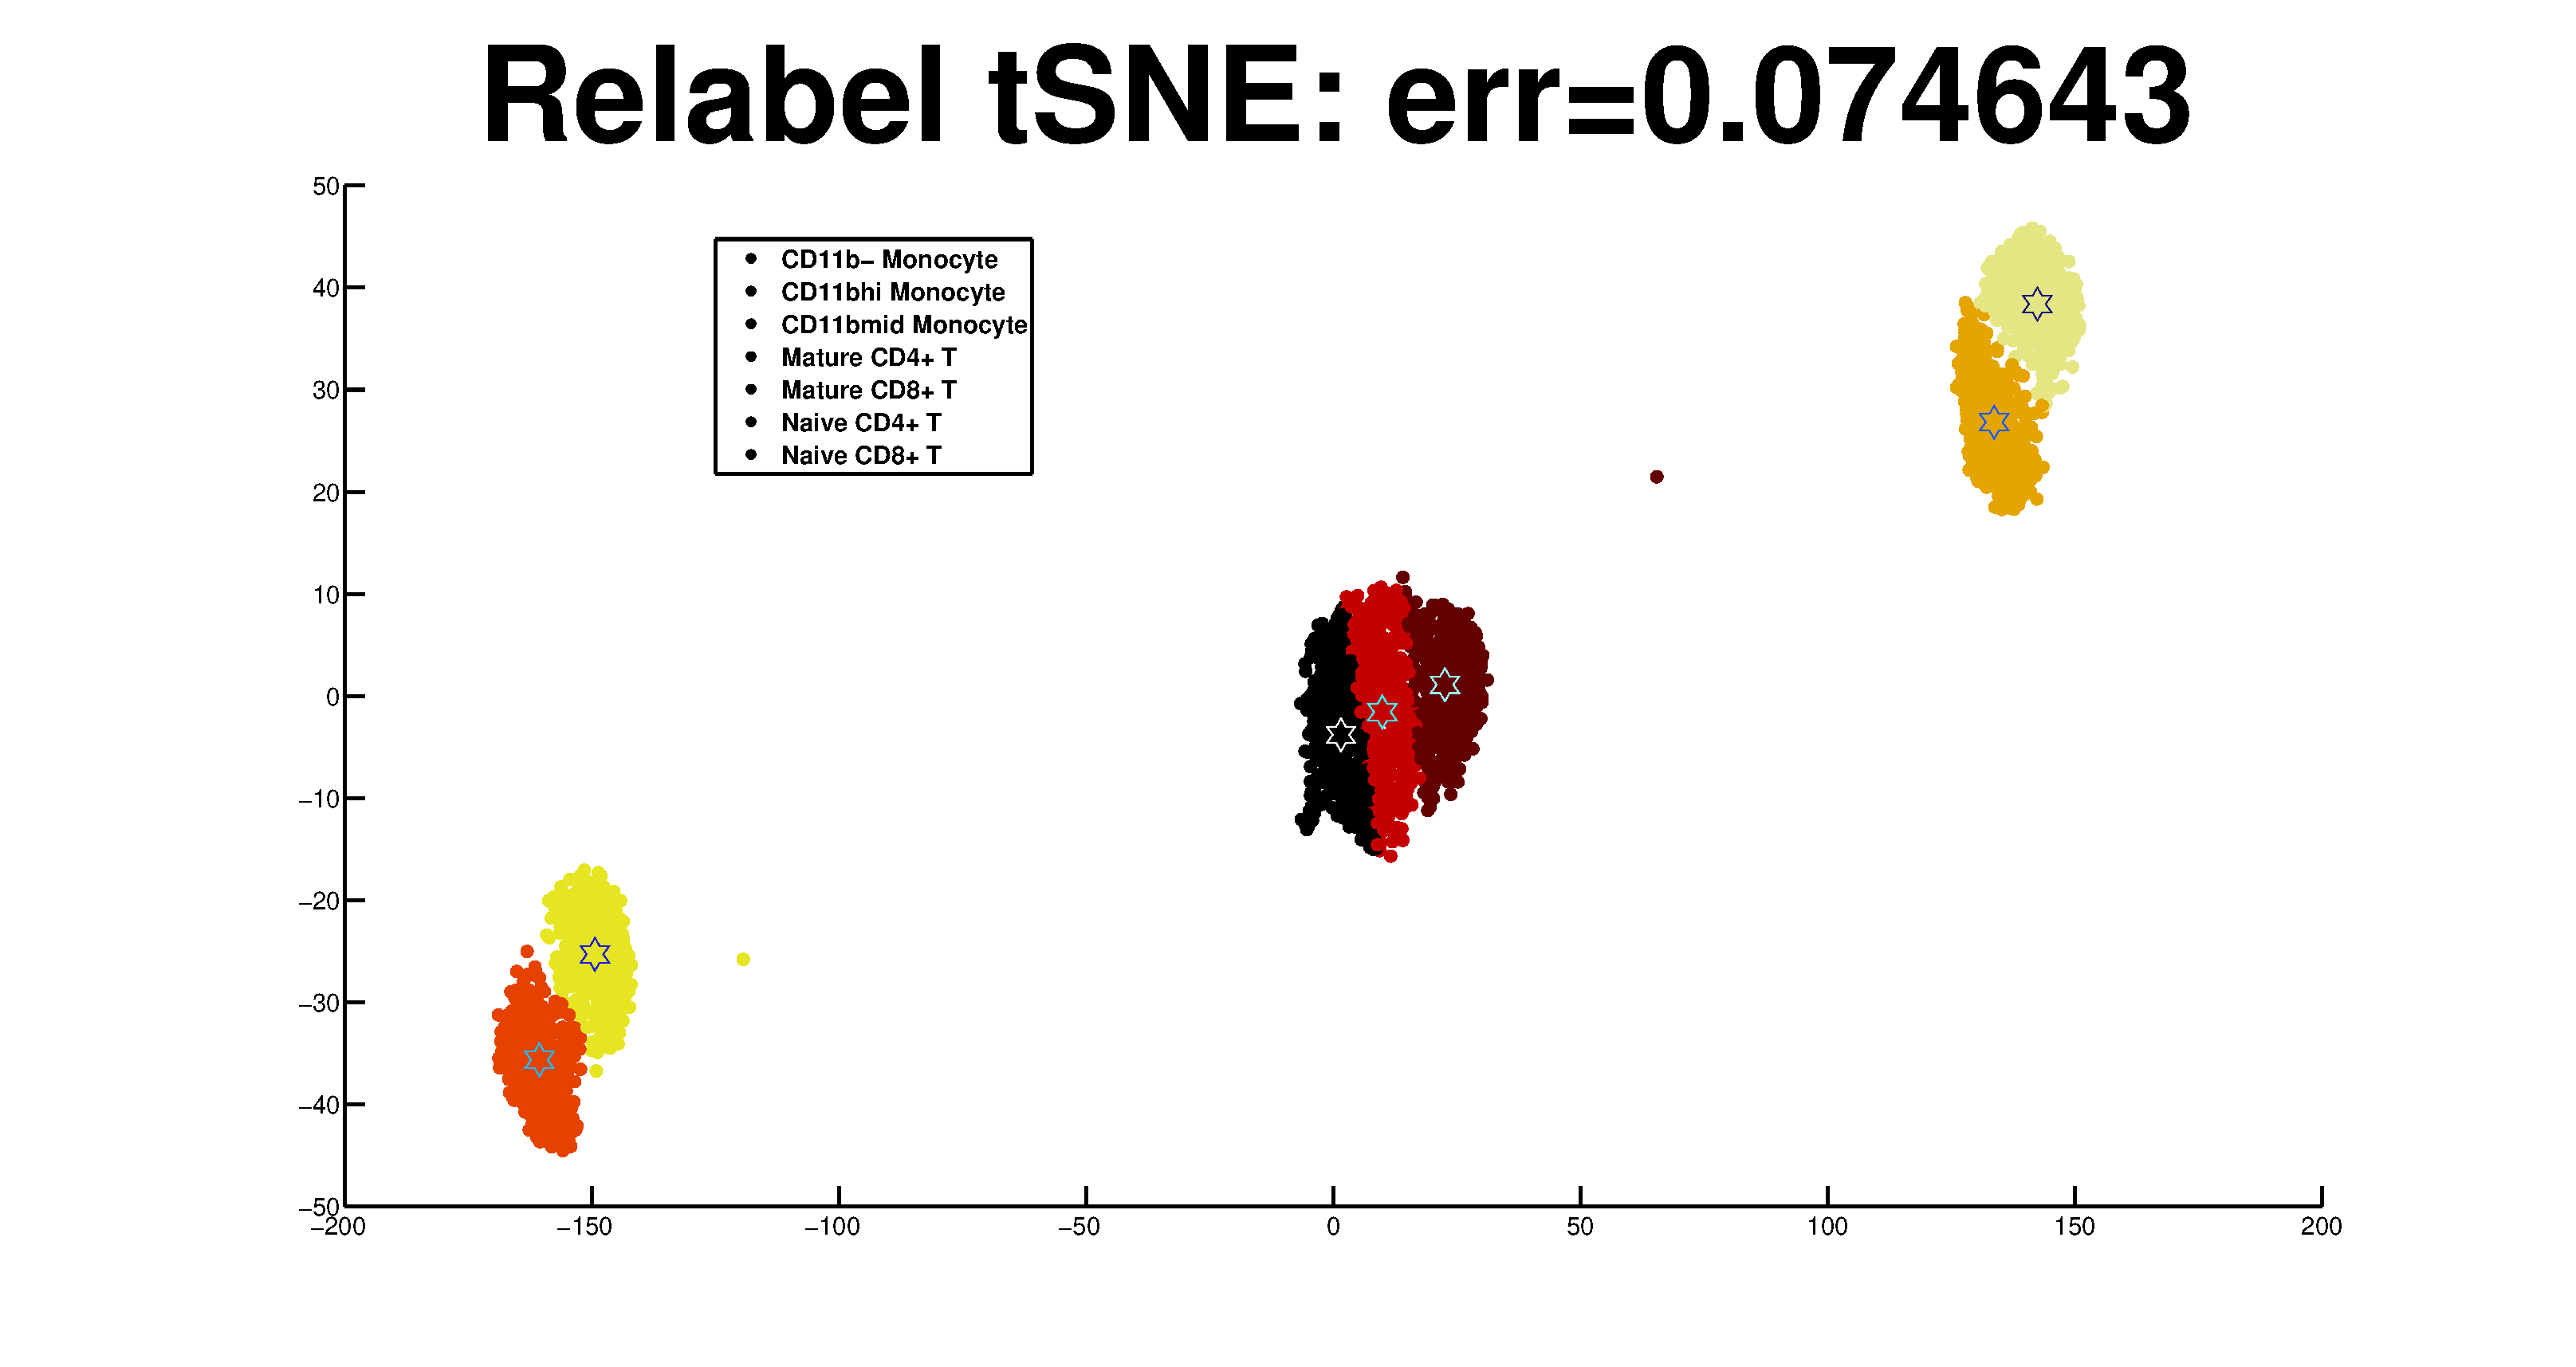
\includegraphics[width=0.47 \columnwidth,  trim = 2.5in 0.5in 1in 2in]{tSNE_Monocytes&TCells_N=400_relabel}}\quad
\end{center}
\caption{tSNE on Monocytes and T Cells with 400 cells per subtype}
\label{tSNEmonocytesandtcells}
\vskip -0.2in
\end{figure}


%s-SNE for all cell types
\begin{figure}[h]
\vskip 0.2in
\begin{center}
\subfloat[Original Labels]{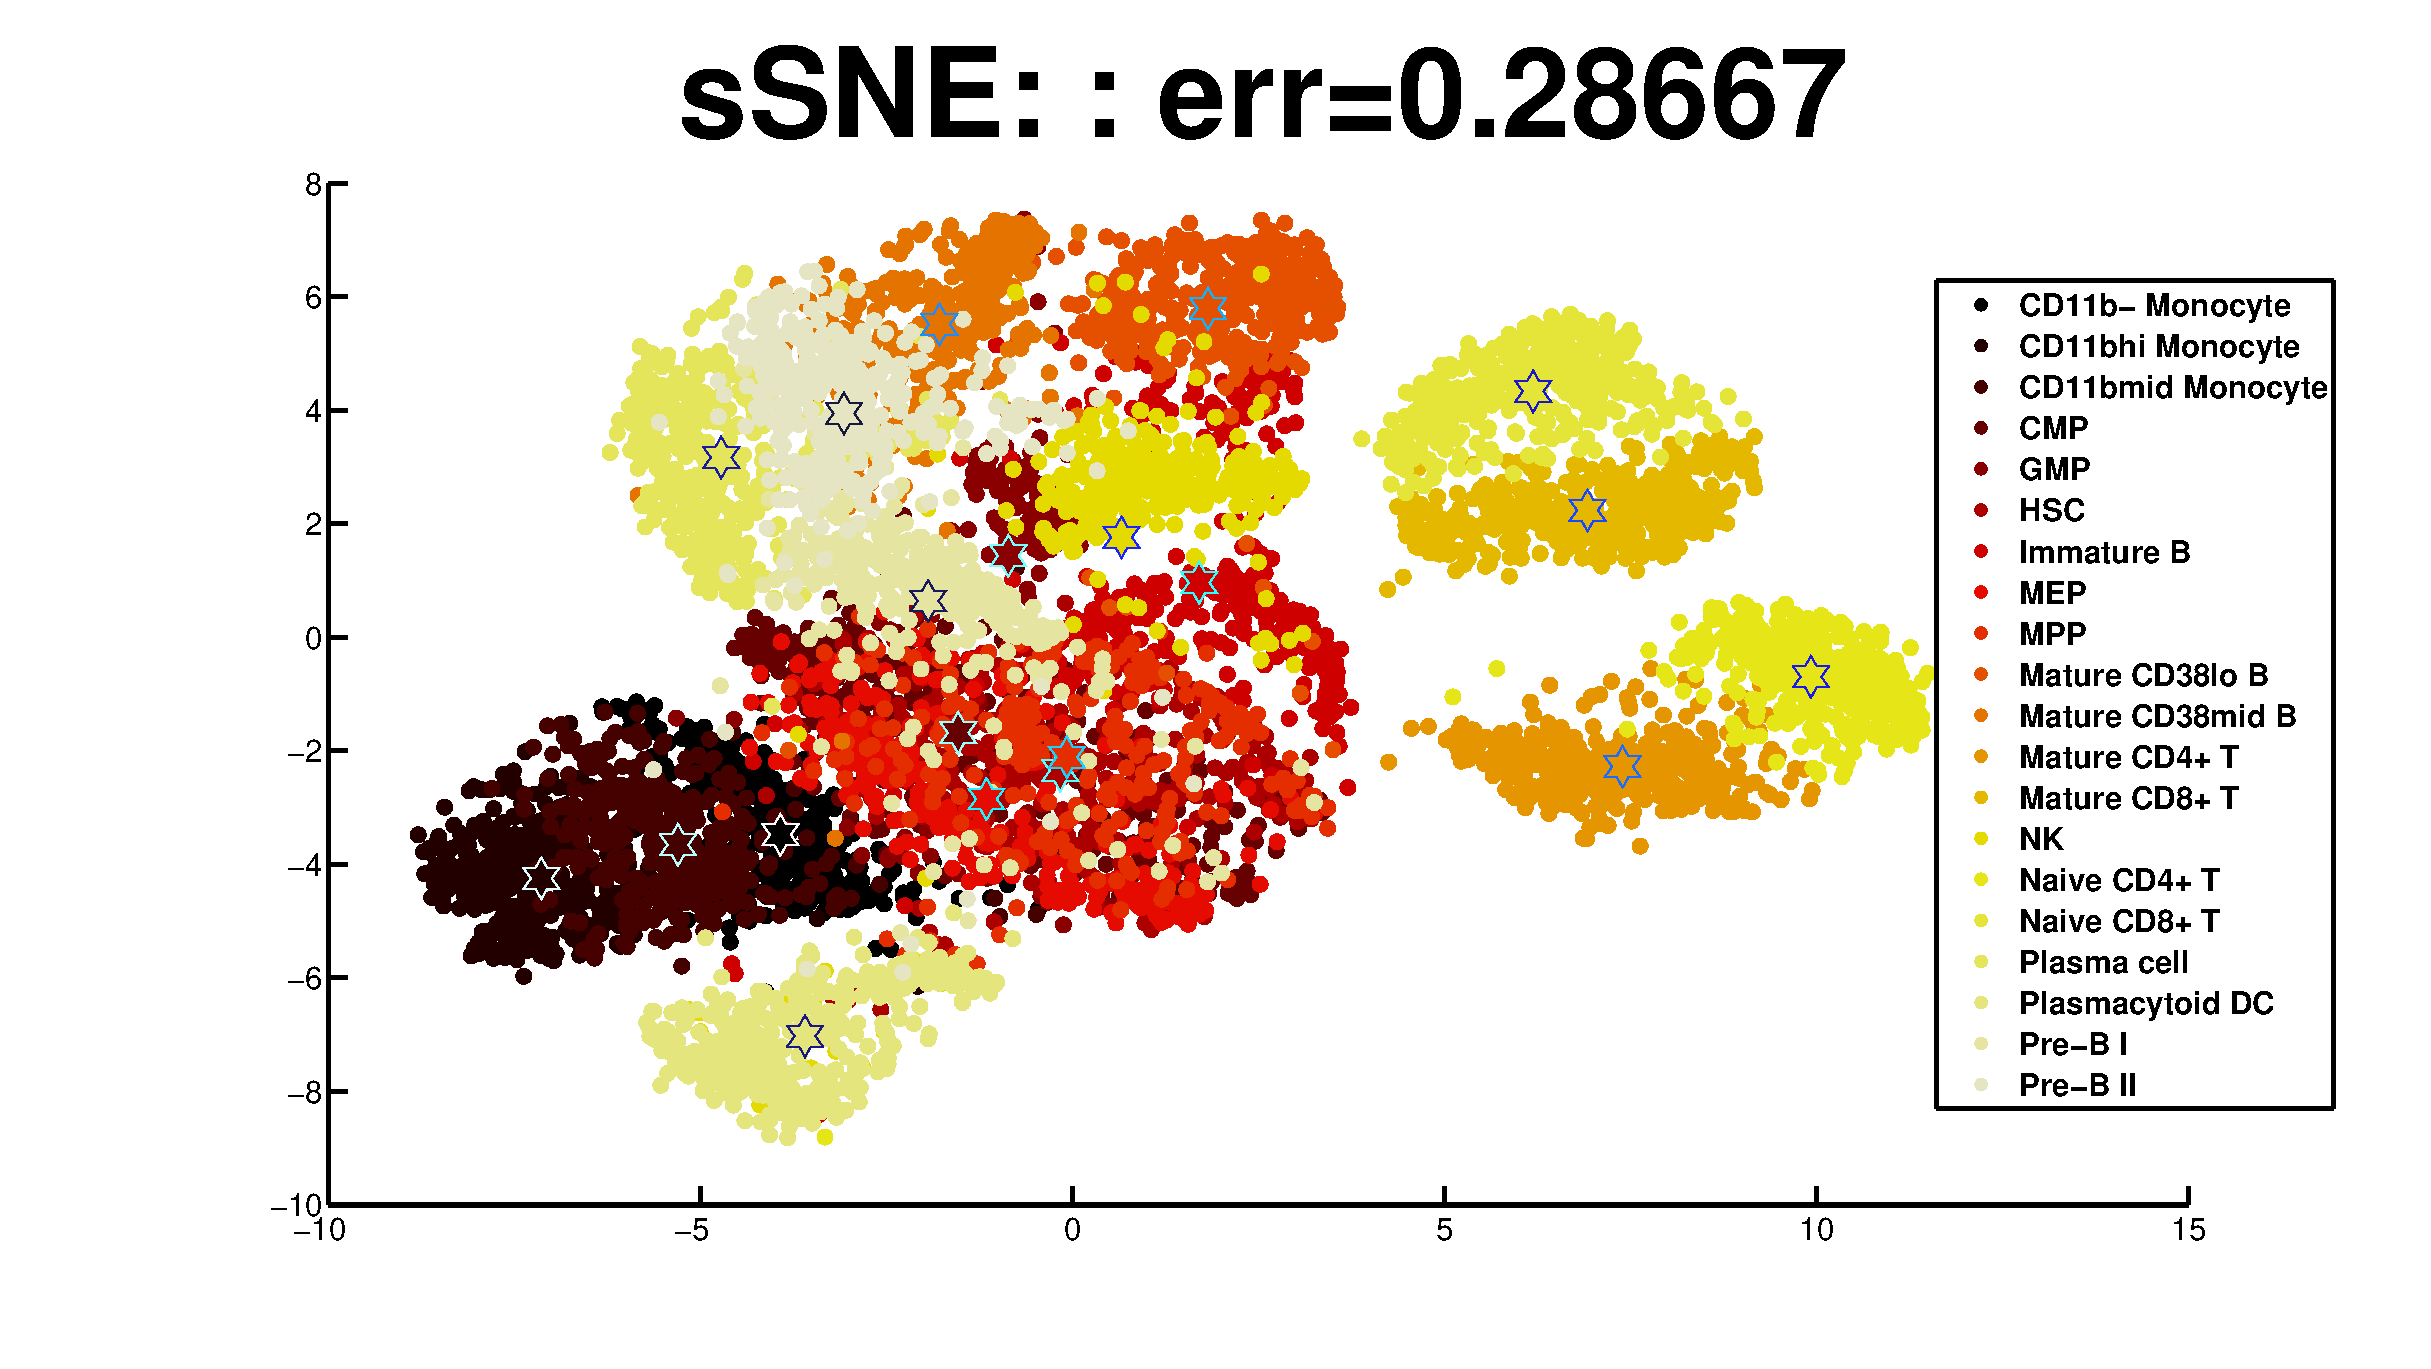
\includegraphics[width=0.47\columnwidth, trim = 2.5in 0.5in 1in 2in]{sSNE_AllCells_N=400}}\quad
\subfloat[New Labels]{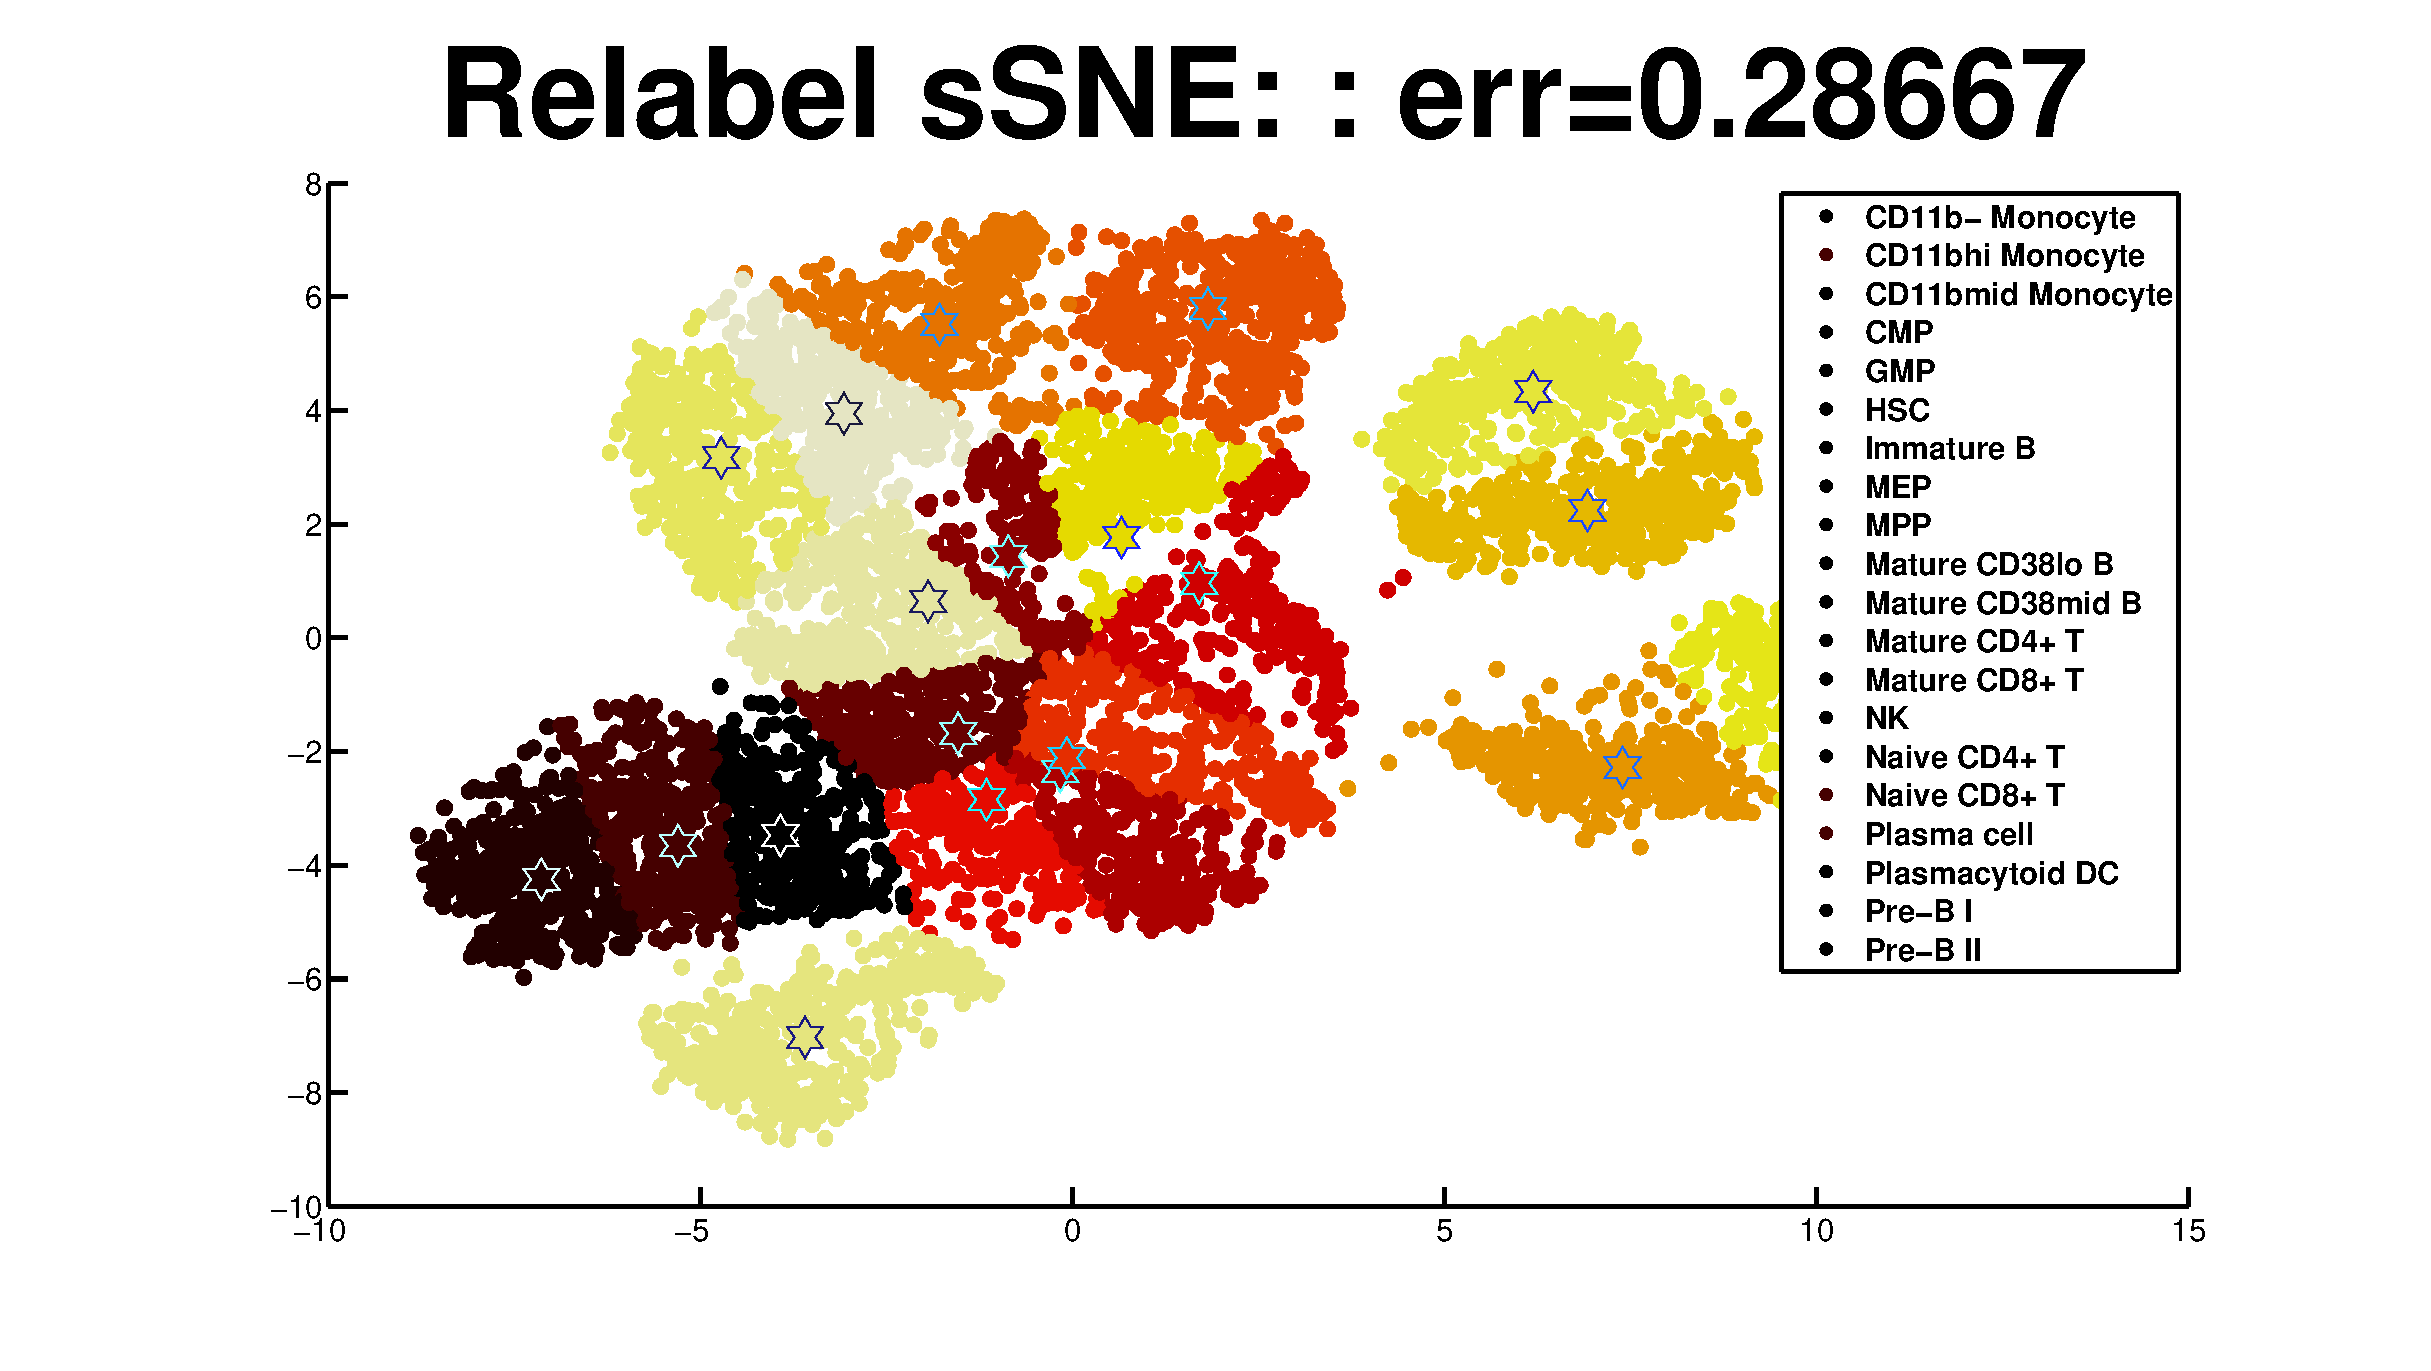
\includegraphics[width=0.47 \columnwidth,  trim = 2.5in 0.5in 1in 2in]{sSNE_AllCells_N=400_relabel}}\quad
\end{center}
\caption{sSNE on all cell subtypes with 400 cells per subtype}
\label{sSNEall}
\vskip -0.2in
\end{figure}

%s-SNE for Monocytes and T Cells
\begin{figure}[h]
\vskip 0.2in
\begin{center}
\subfloat[Original Labels]{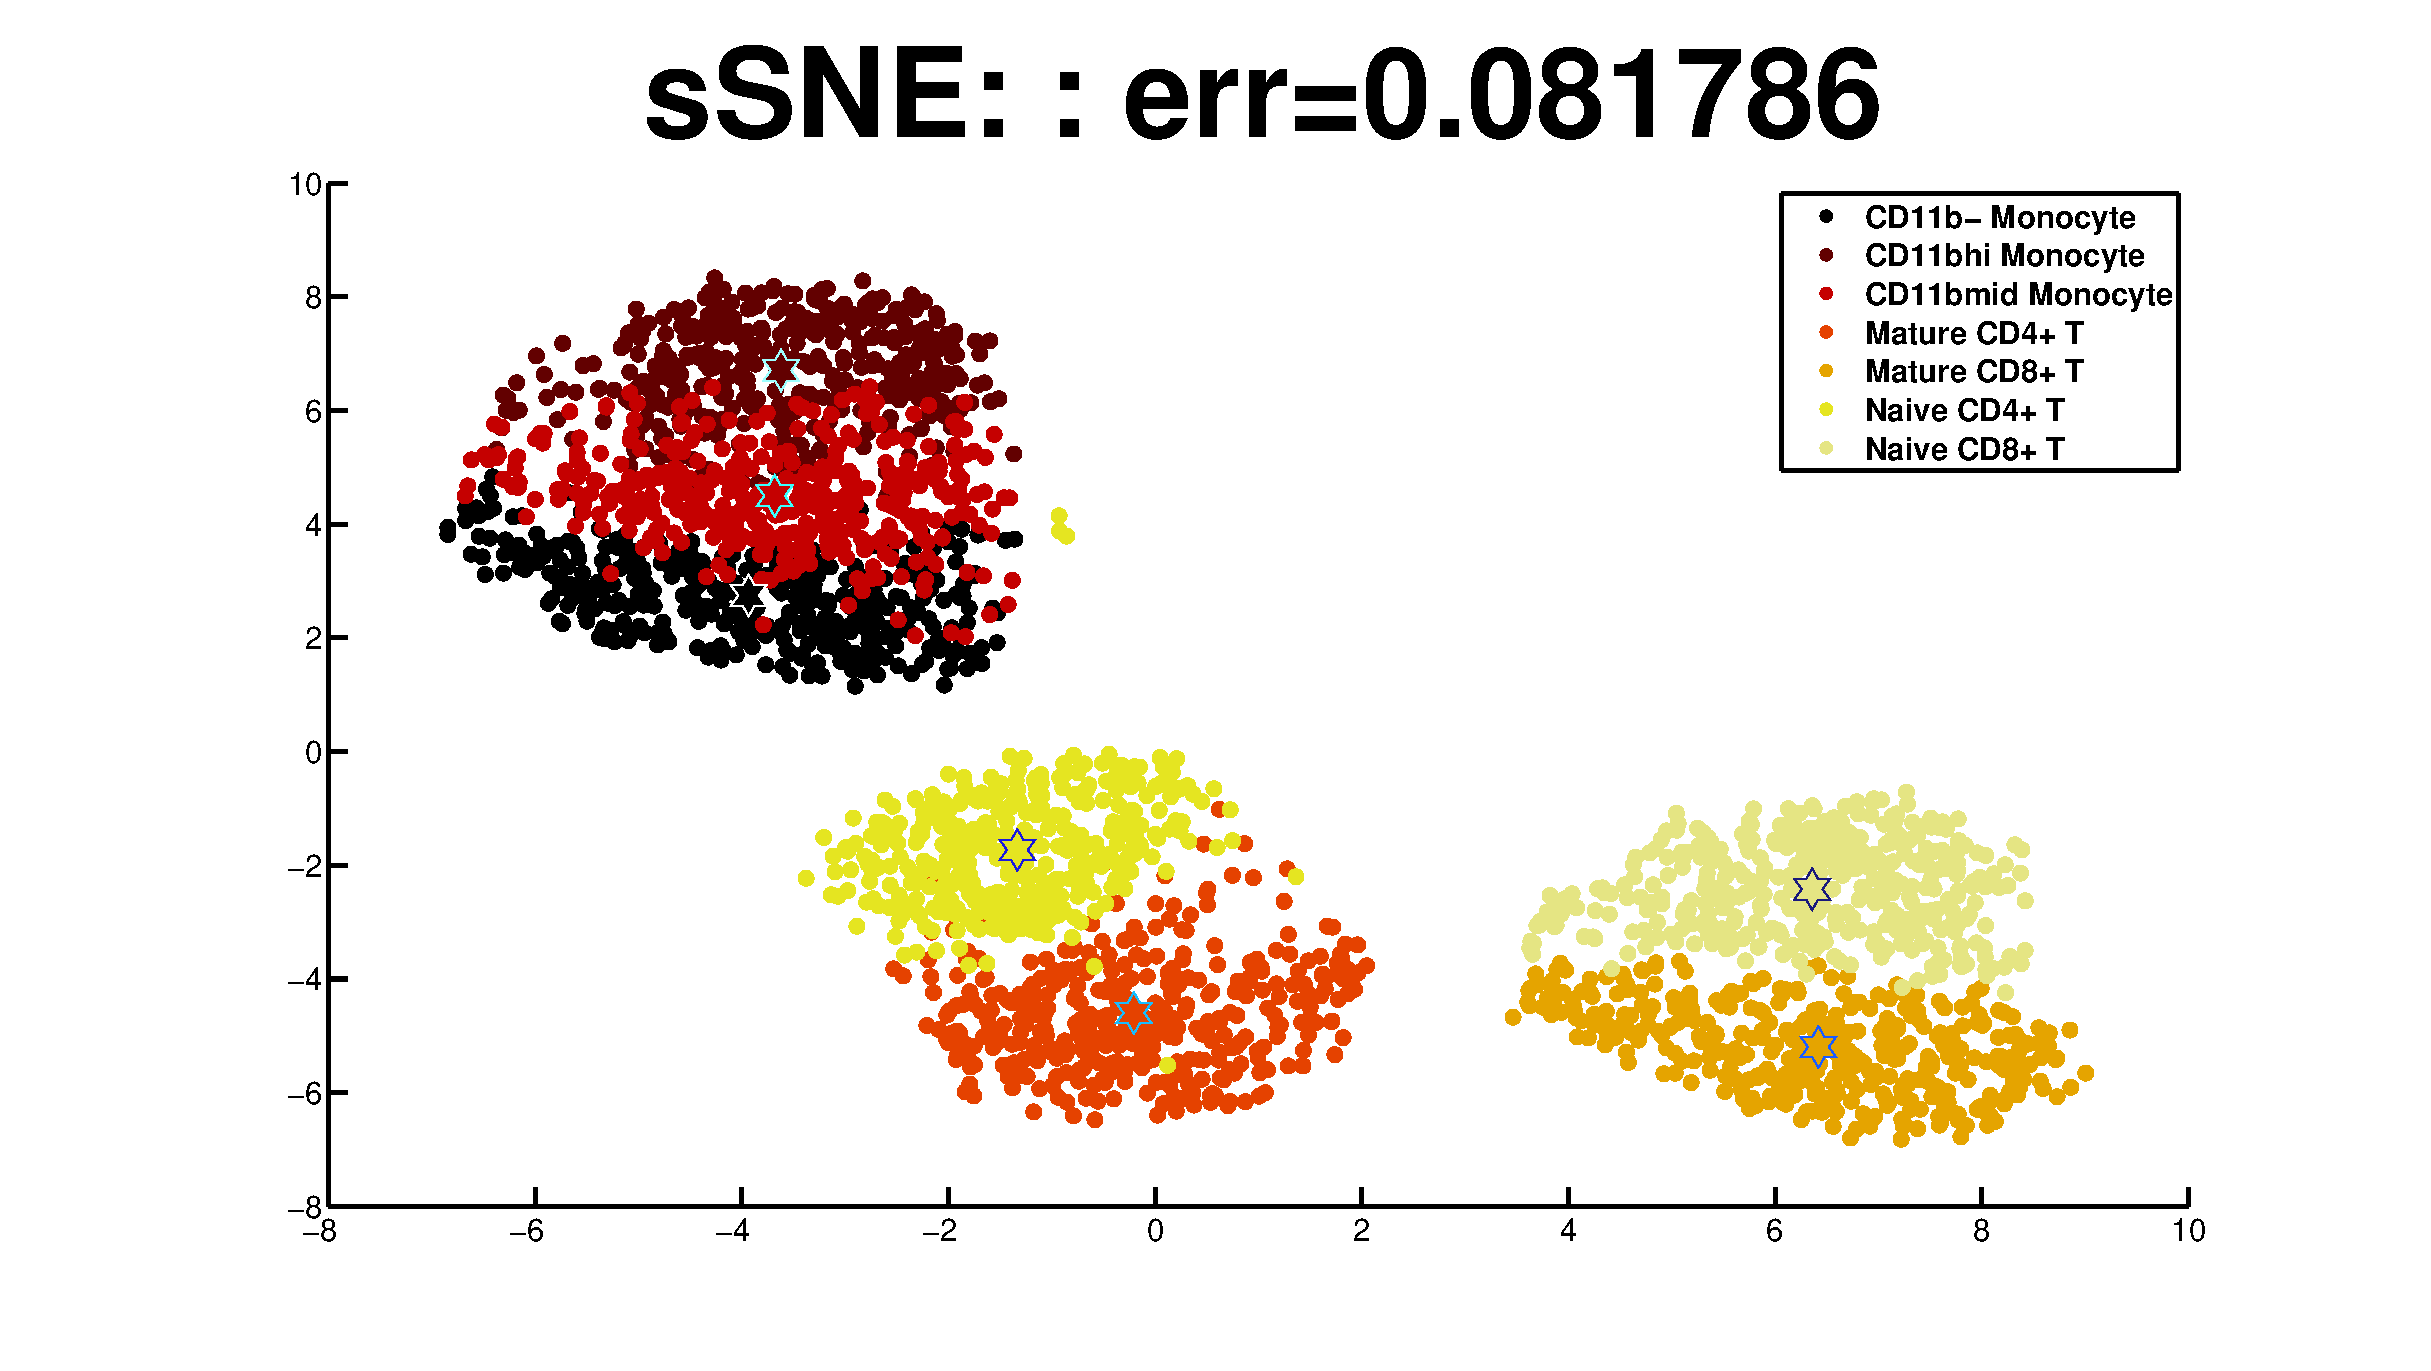
\includegraphics[width=0.47\columnwidth, trim = 2.5in 0.5in 1in 2in]{sSNE_Monocytes&TCells_N=400}}\quad
\subfloat[New Labels]{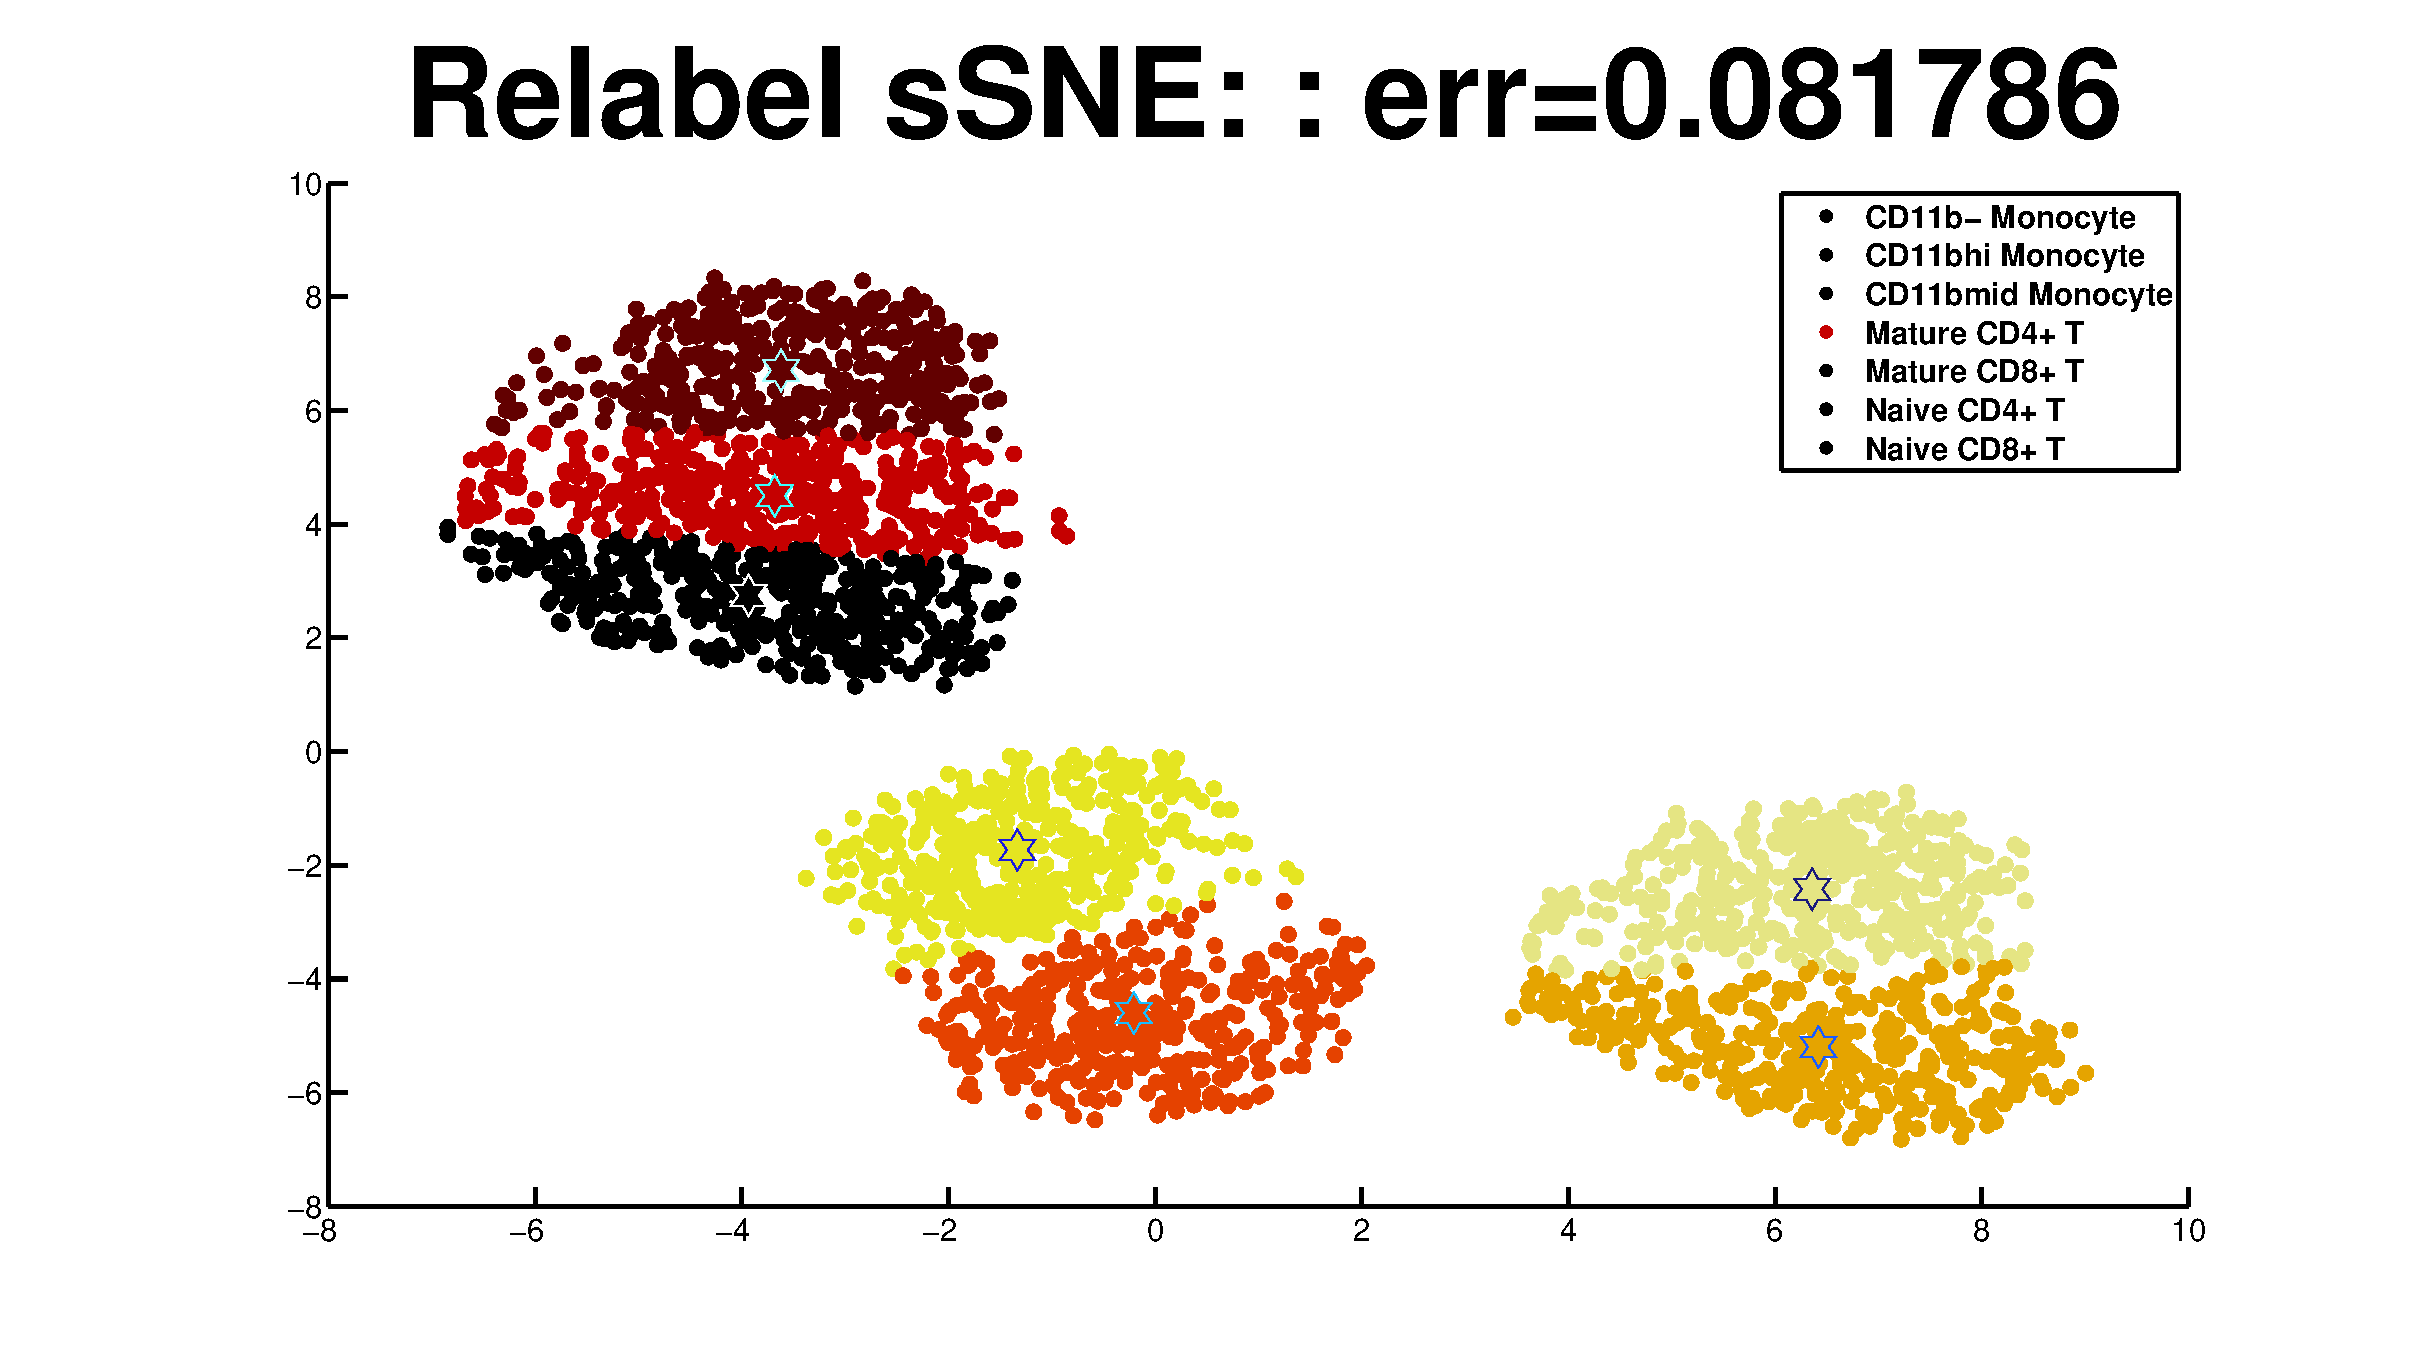
\includegraphics[width=0.47 \columnwidth,  trim = 2.5in 0.5in 1in 2in]{sSNE_Monocytes&TCells_N=400_relabel}}\quad
\end{center}
\caption{sSNE on Monocytes and T Cells with 400 cells per subtype}
\label{sSNEmonocytesandtcells}
\vskip -0.2in
\end{figure}

We now look to EE, the last of the nonlinear methods we are considering. Once again, we take a sample of 400 cells from (i) all cell types and (ii) Monocytes and T Cells.

%EE for all cell types
\begin{figure}[h]
\vskip 0.2in
\begin{center}
\subfloat[Original Labels]{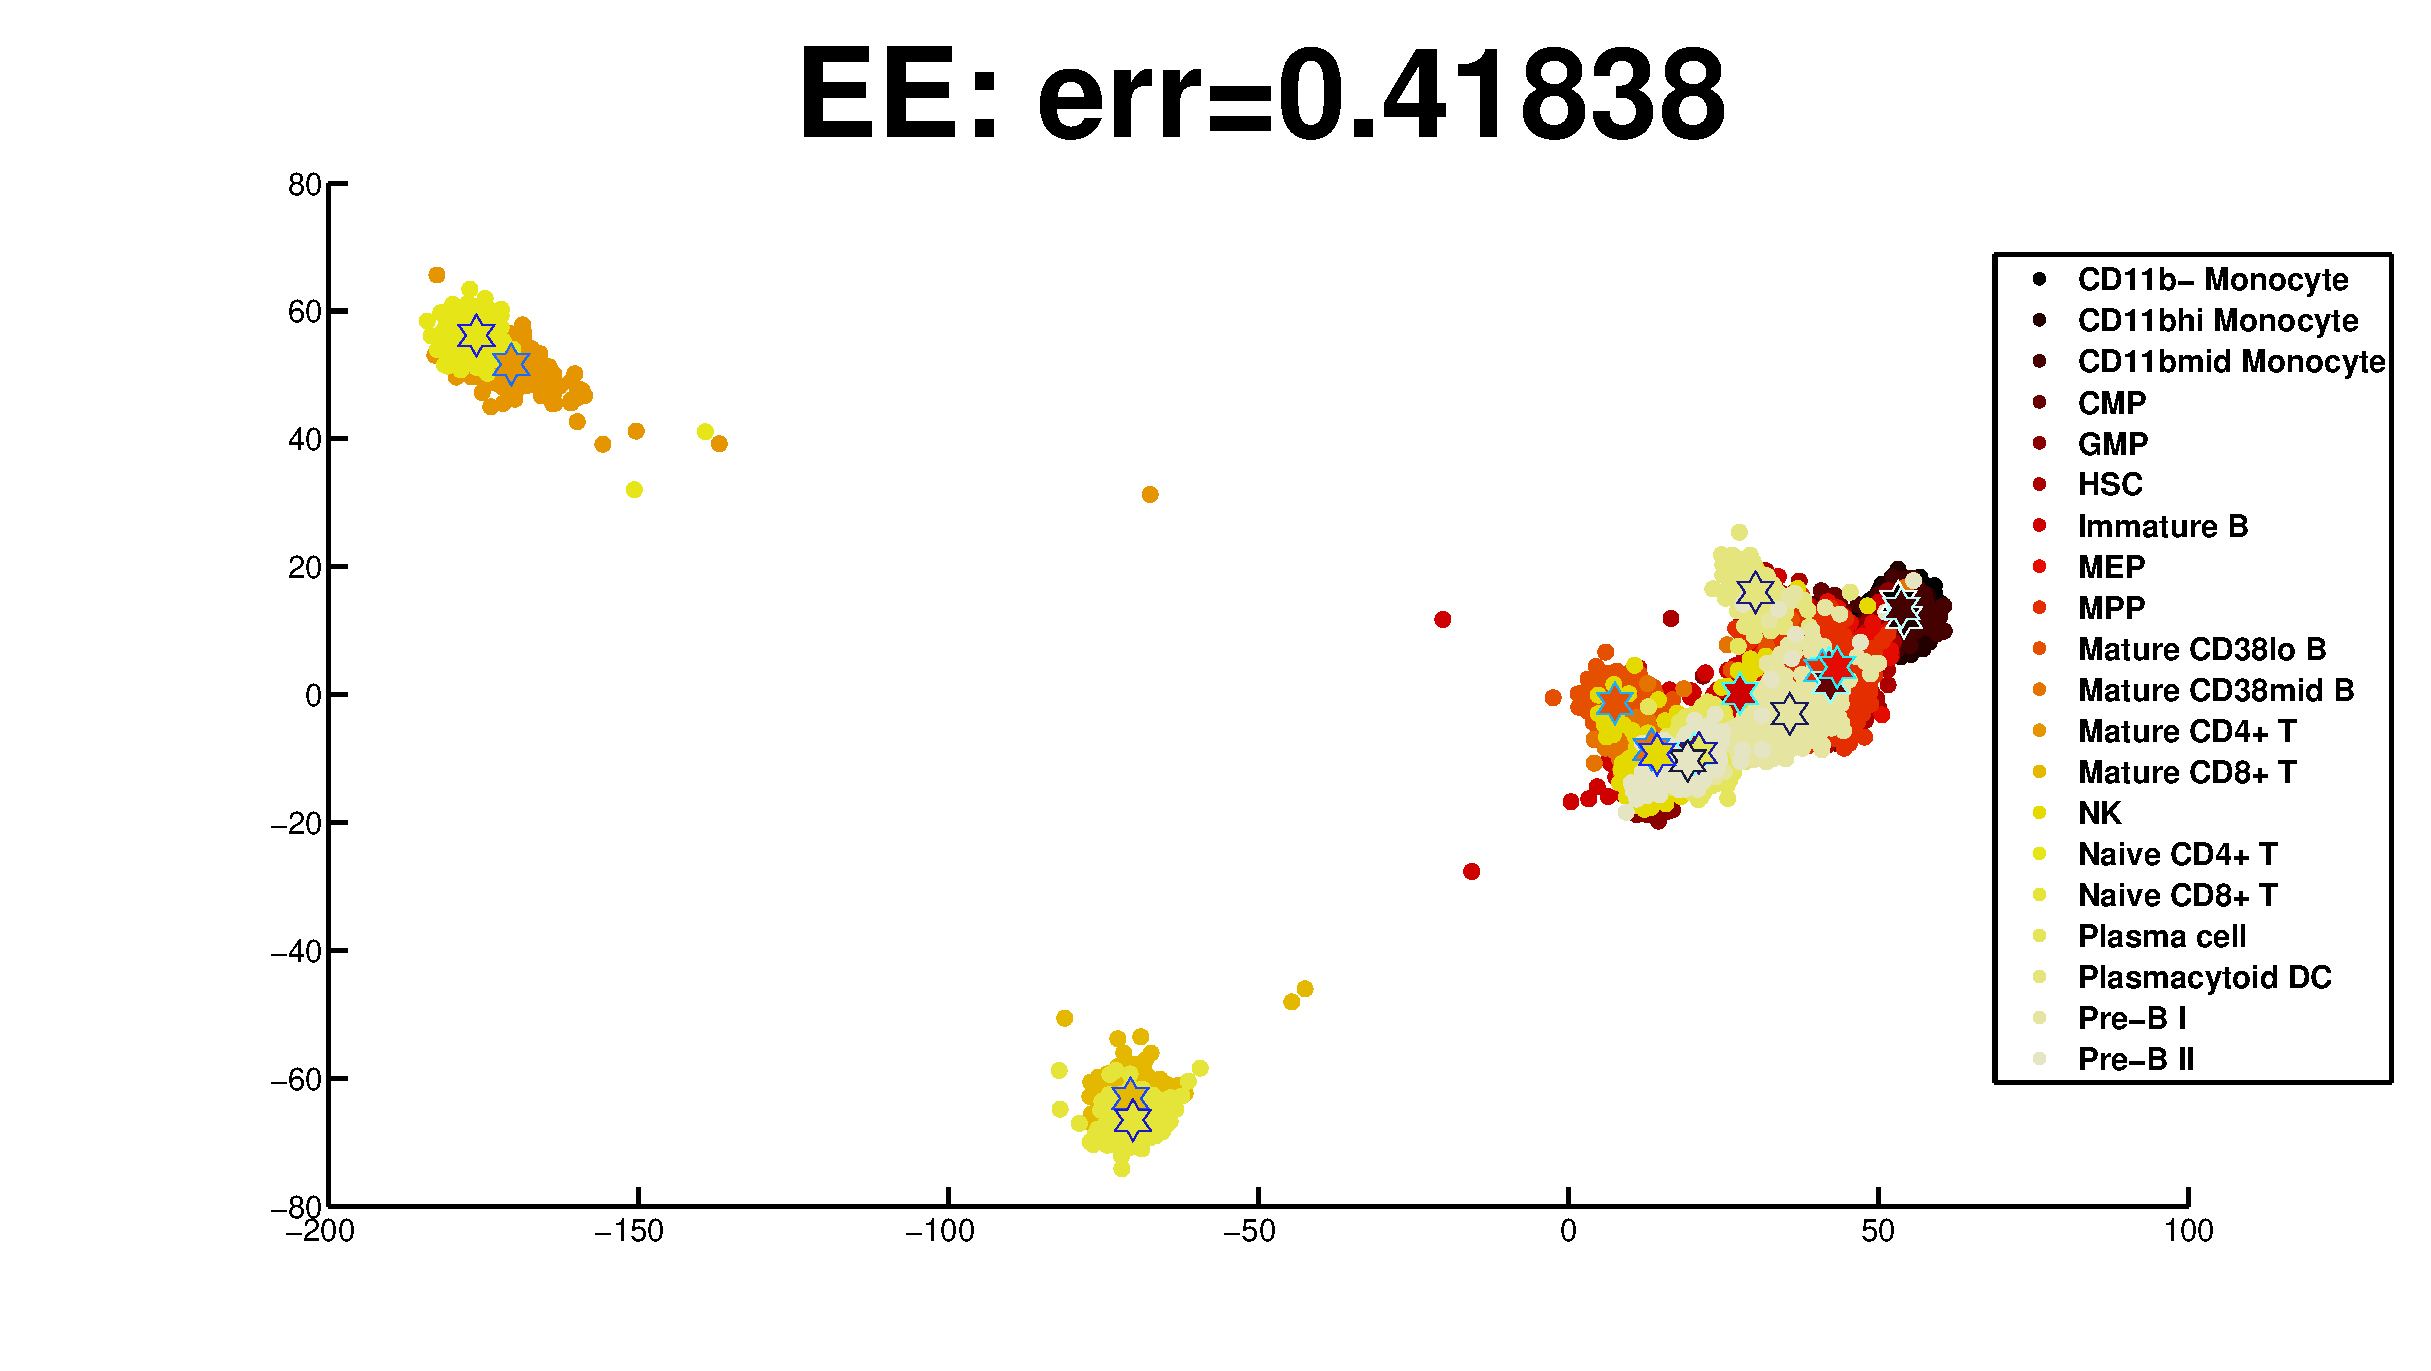
\includegraphics[width=0.47\columnwidth, trim = 2.5in 0.5in 1in 2in]{EE_AllCells_N=400}}\quad
\subfloat[New Labels]{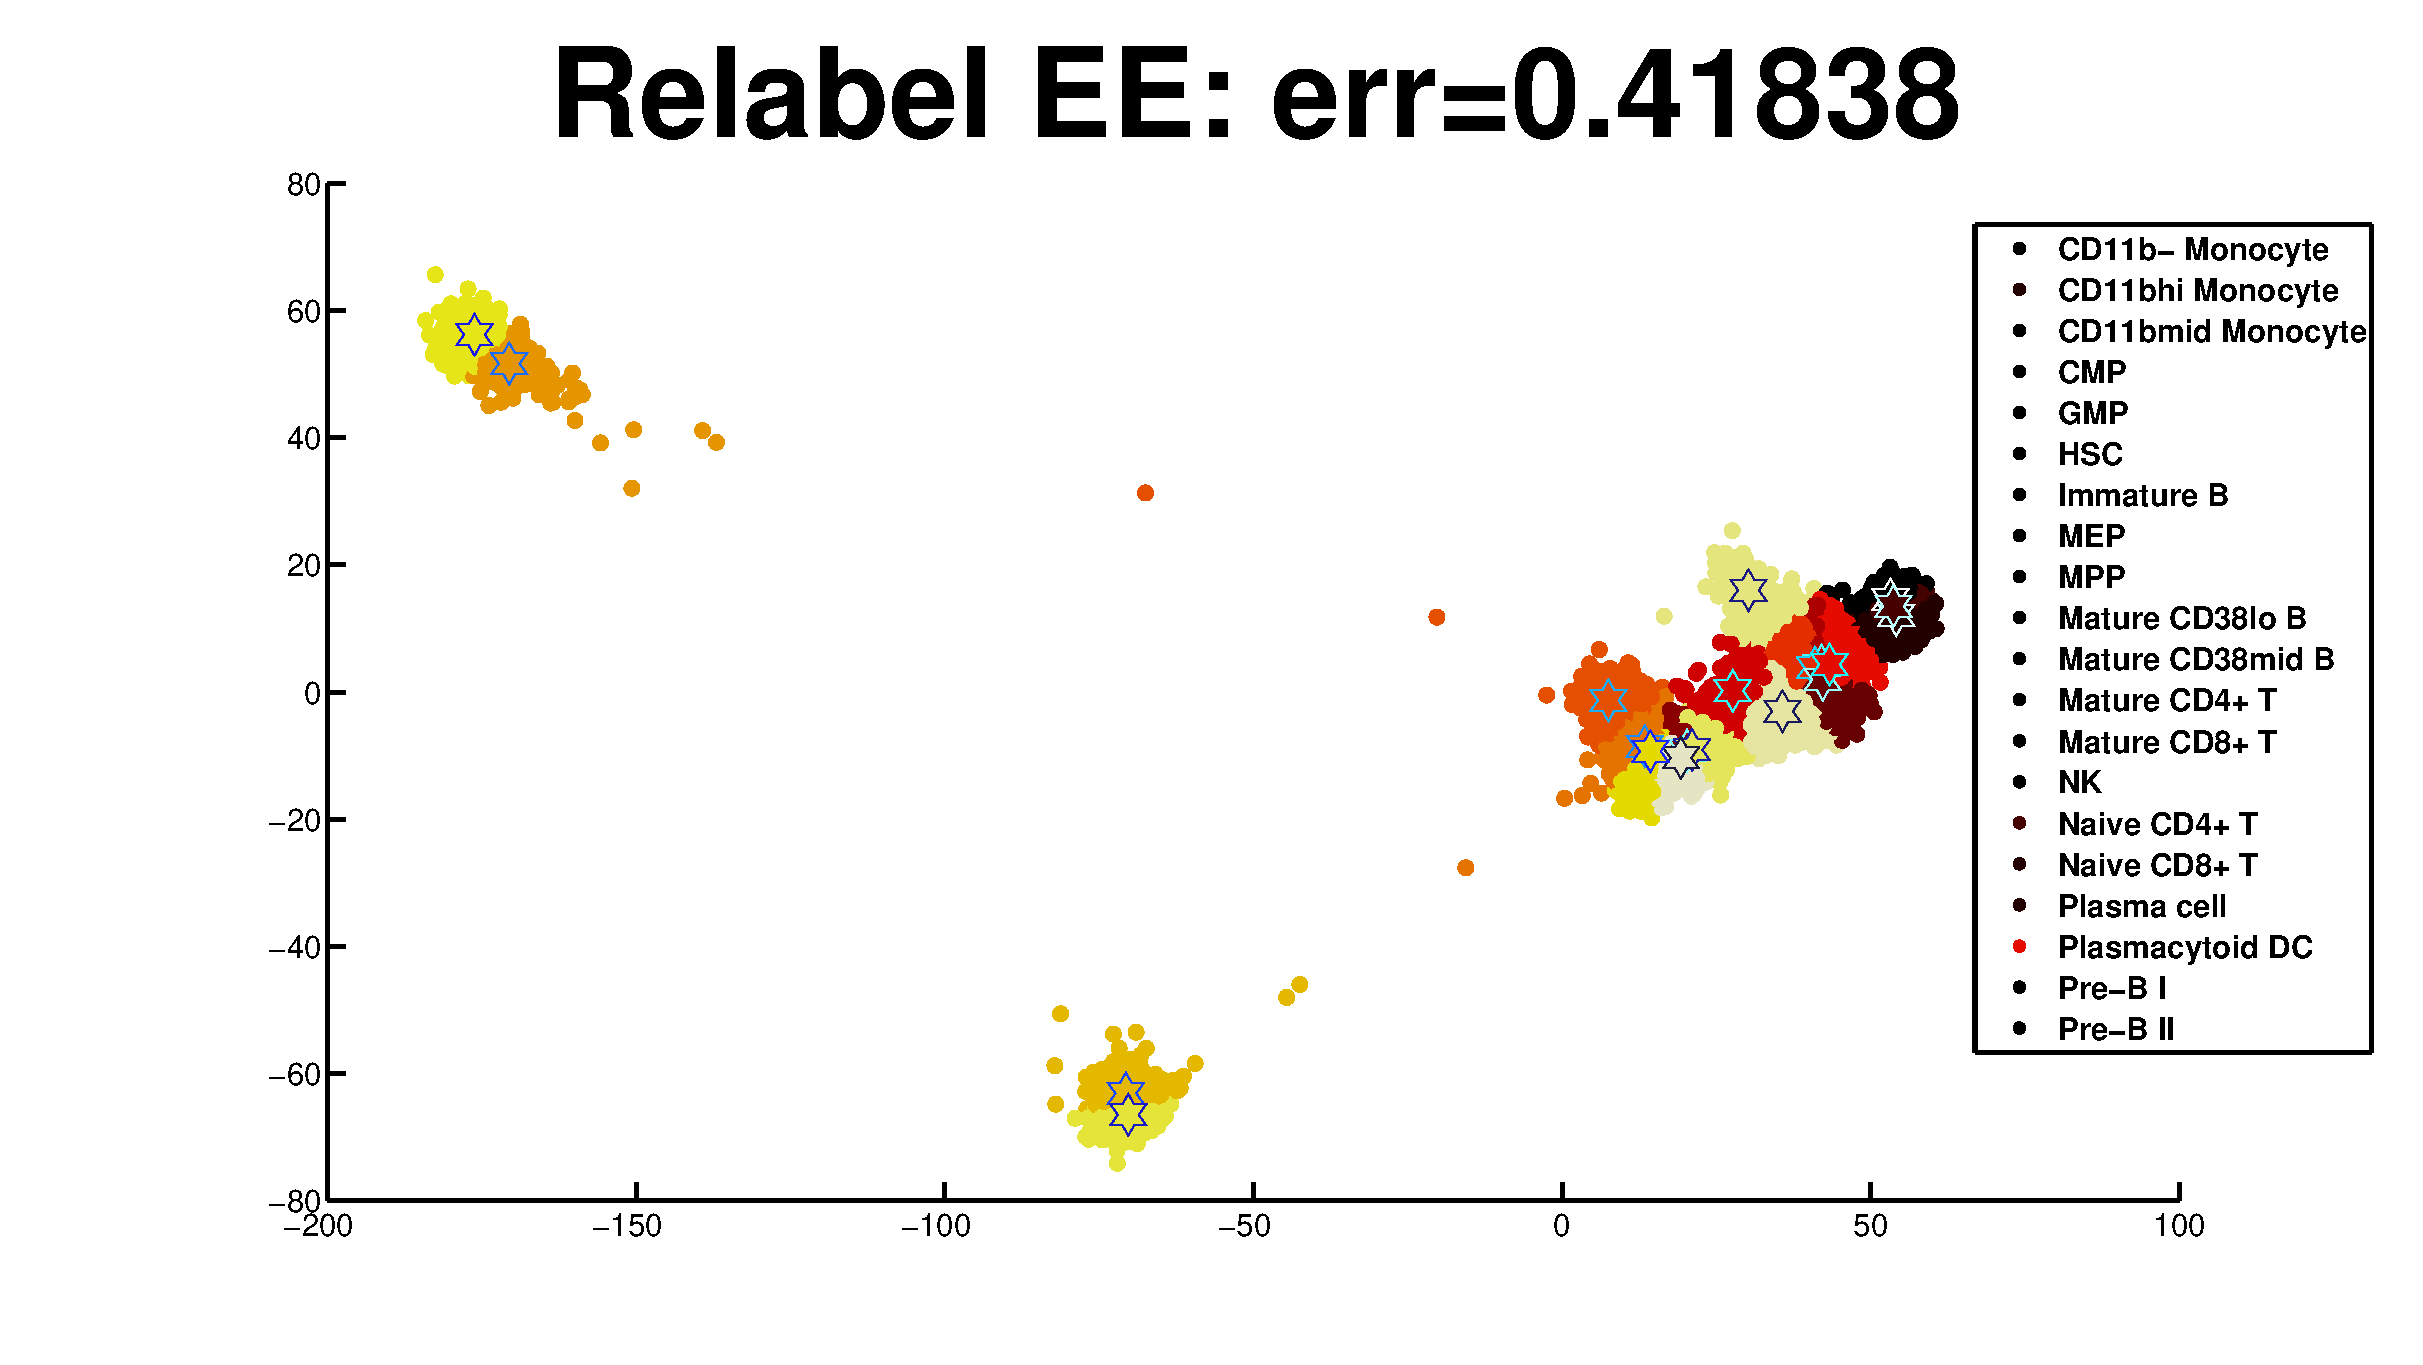
\includegraphics[width=0.47 \columnwidth,  trim = 2.5in 0.5in 1in 2in]{EE_AllCells_N=400_relabel}}\quad
\end{center}
\caption{EE on Monocytes and T Cells with 400 cells per subtype}
\label{EEall}
\vskip -0.2in
\end{figure}


% EE for monocytes and T Cells
\begin{figure}[h]
\vskip 0.2in
\begin{center}
\subfloat[Original Labels]{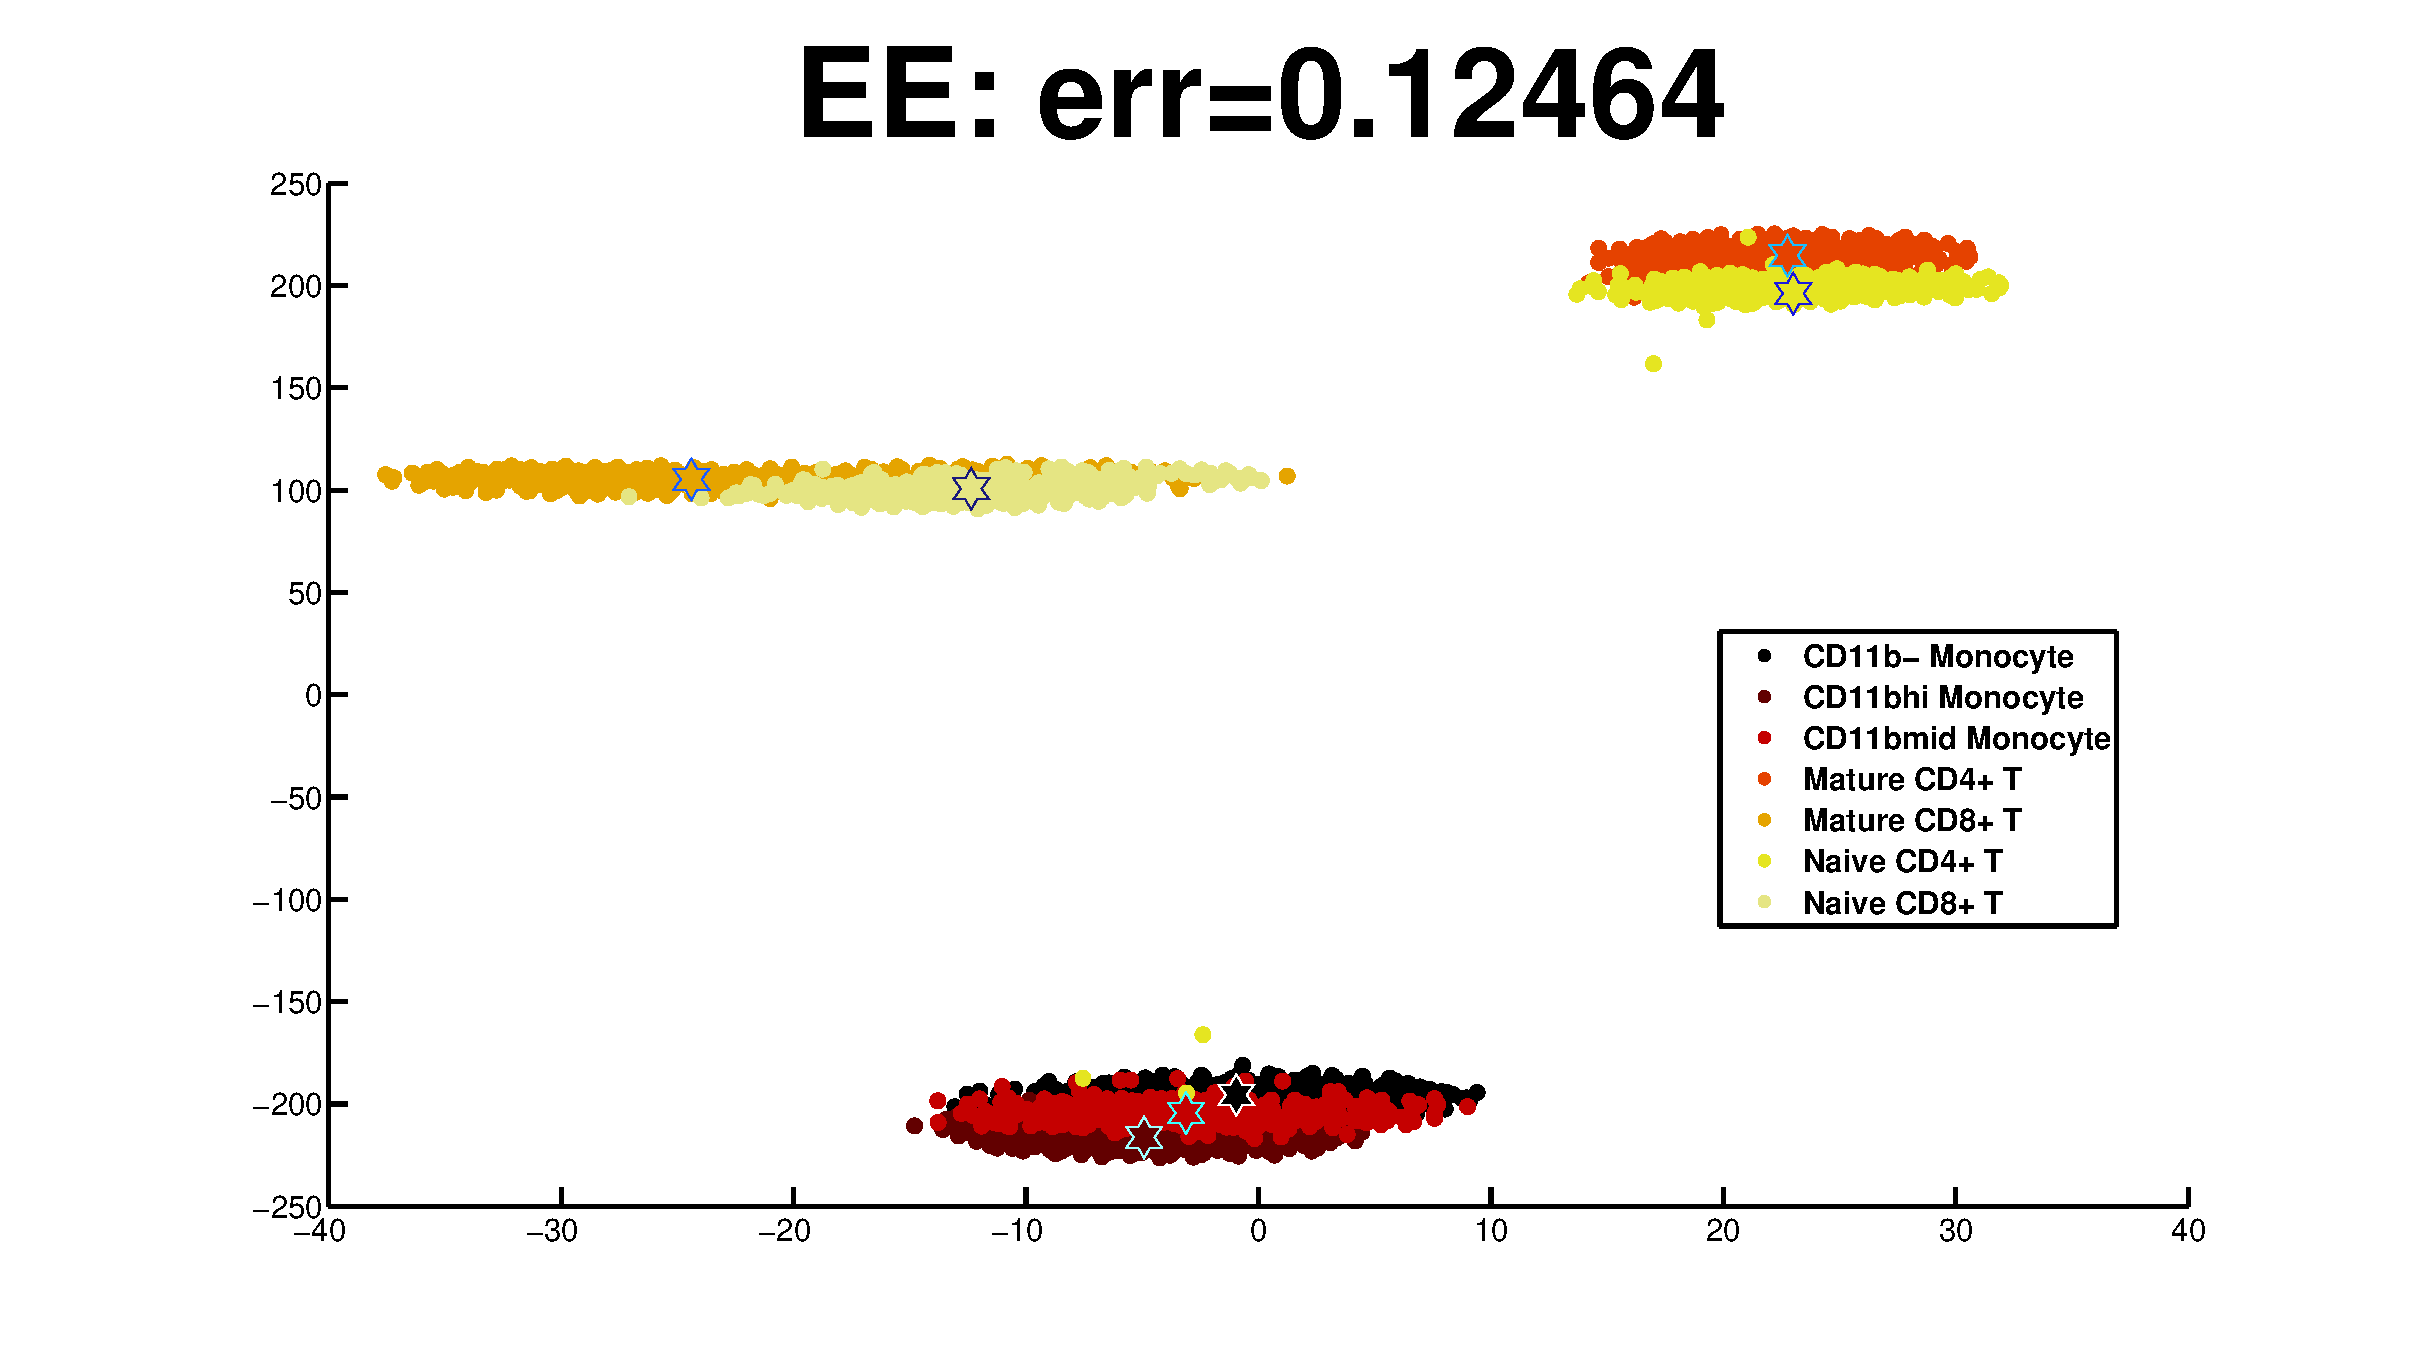
\includegraphics[width=0.47\columnwidth, trim = 2.5in 0.5in 1in 2in]{EE_Monocytes&TCells_N=400}}\quad
\subfloat[New Labels]{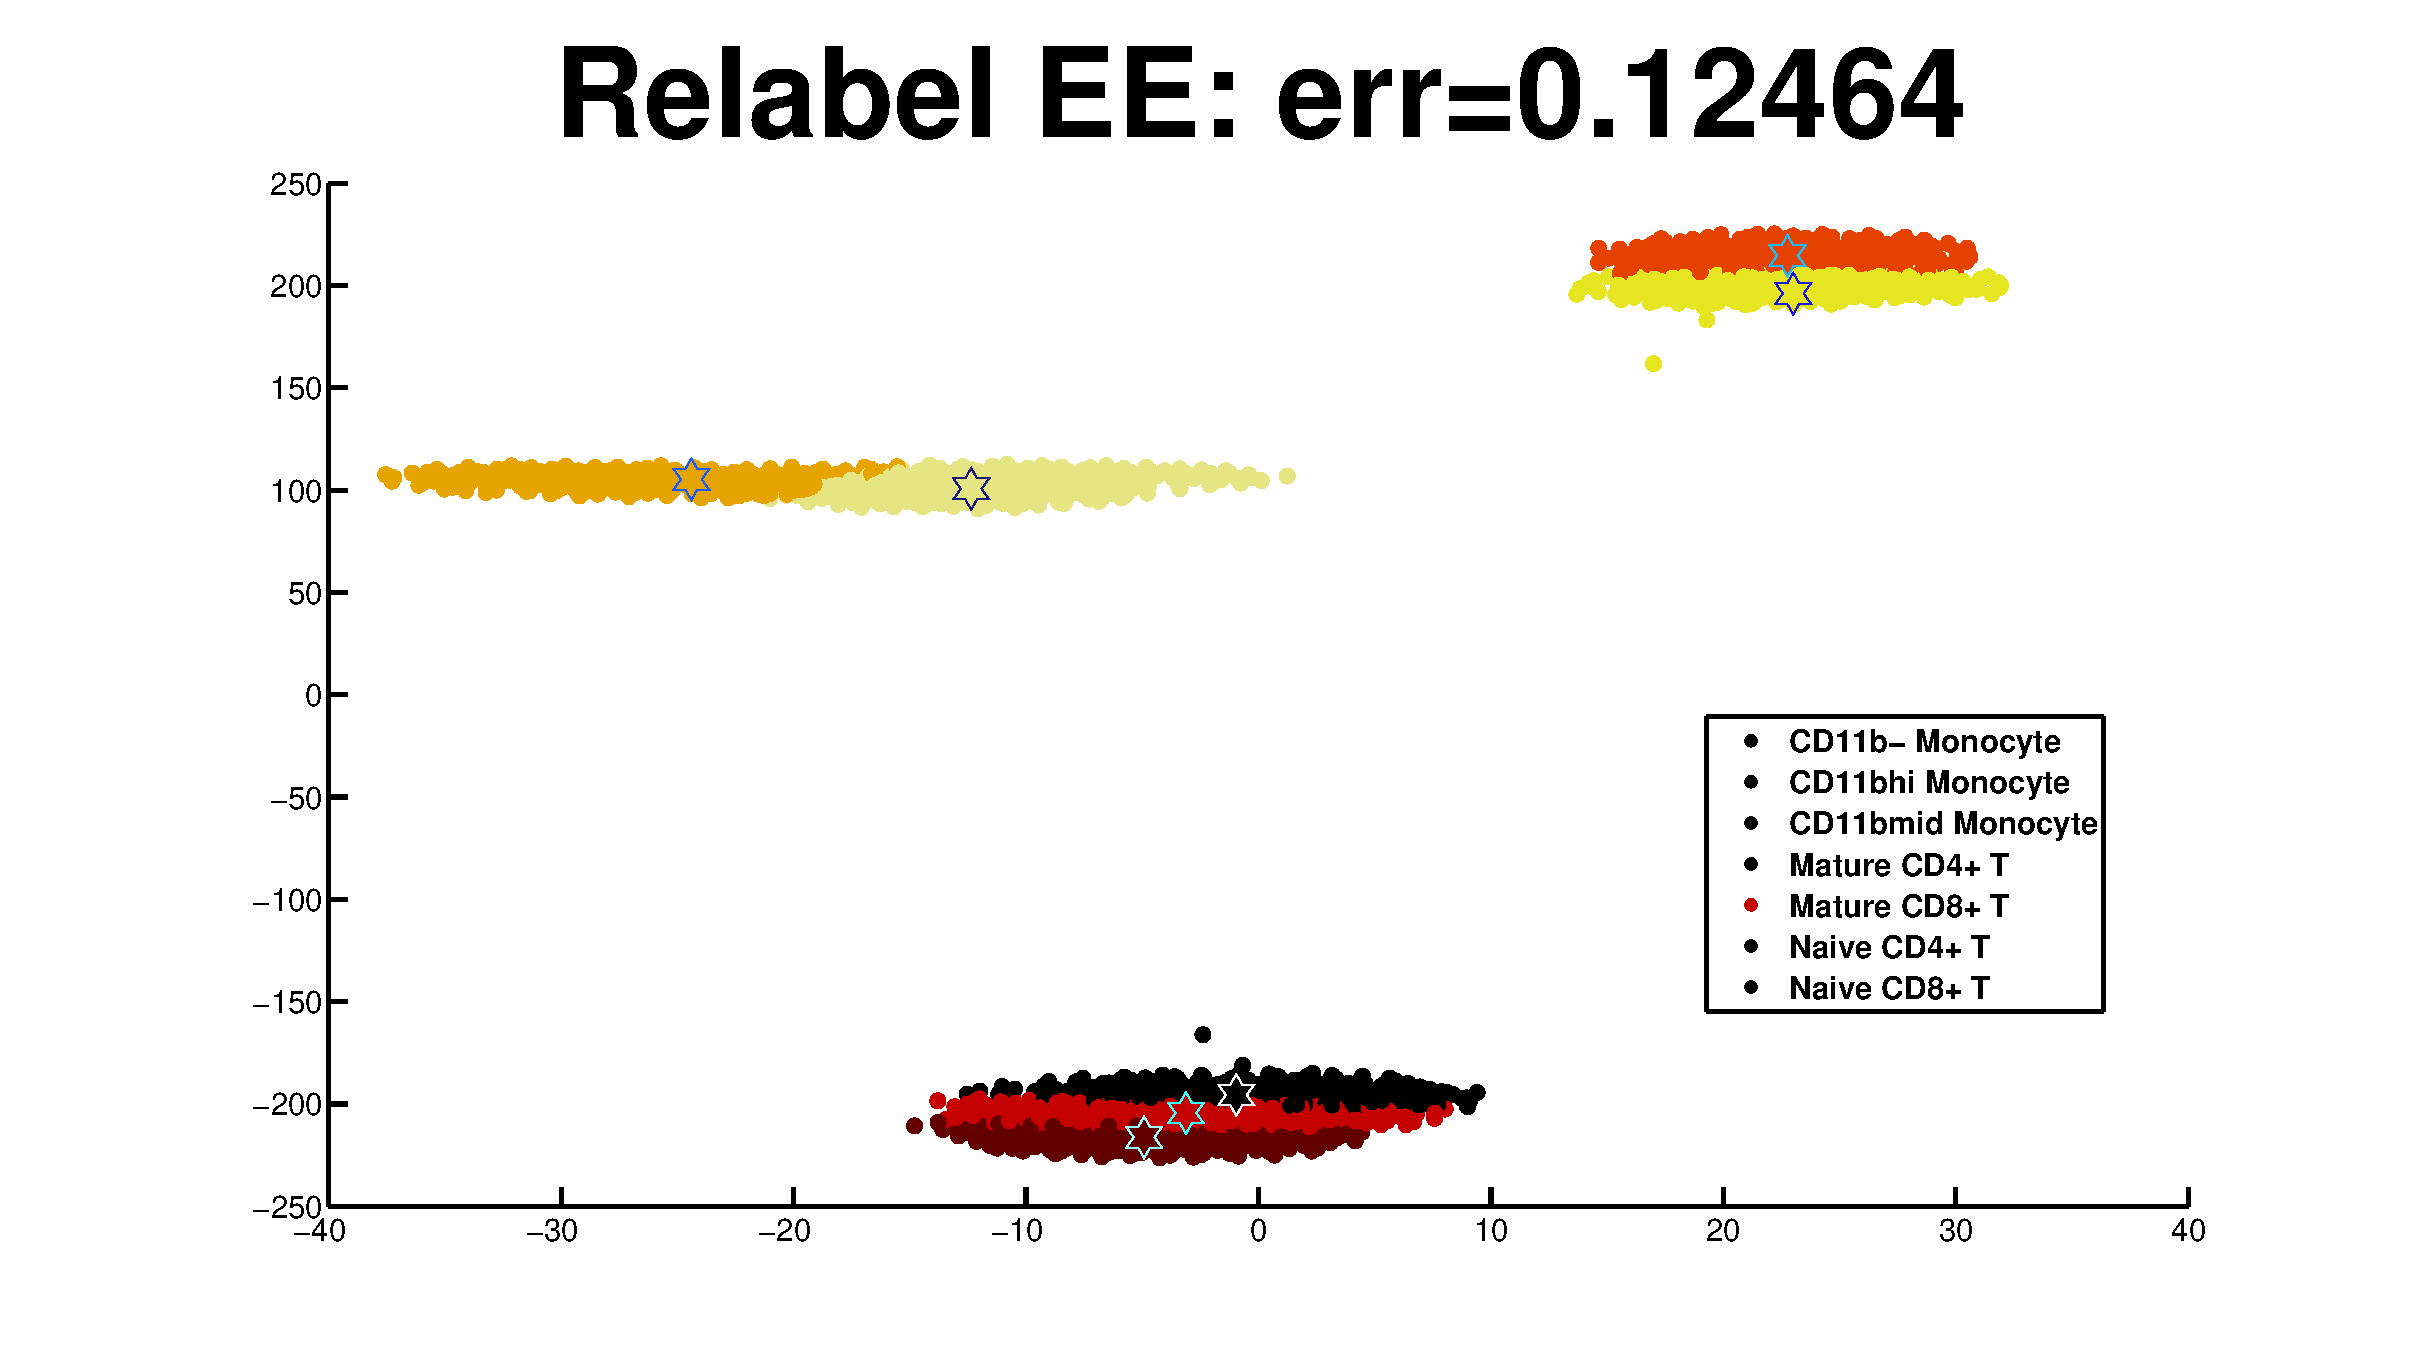
\includegraphics[width=0.47 \columnwidth,  trim = 2.5in 0.5in 1in 2in]{EE_Monocytes&TCells_N=400_relabel}}\quad
\end{center}
\caption{EE on Monocytes and T Cells with 400 cells per subtype}
\label{EEmonocytesandtcells}
\vskip -0.2in
\end{figure}

Table~\ref{tableErrors} summarizes the errors for the different algorithms.

\begin{table}[tb]
\caption{Algorithm Errors}
\label{tableErrors}
\vskip 0.15in
\begin{center}
\begin{small}
\begin{sc}
\begin{tabular}{lcccr}
\hline
\abovespace\belowspace
Algorithm & All Cells & Monocytes \& T Cells \\
\hline
\abovespace
PCA	& 62.18\% & 48.42\%  \\
tSNE 	& 24.33\%  & 7.46\%\\ 
sSNE	& 28.67 \%  & 8.18\%\\
\belowspace
EE		& 41.84\% &12.46\% \\
\hline
\end{tabular}
\end{sc}
\end{small}
\end{center}
\vskip -0.1in
\end{table}

\subsection{Citations and References} 

Please use APA reference format regardless of your formatter
or word processor. If you rely on the \LaTeX\/ bibliographic 
facility, use {\tt natbib.sty} and {\tt icml2012.bst} 
included in the style-file package to obtain this format.

Citations within the text should include the authors' last names and
year. If the authors' names are included in the sentence, place only
the year in parentheses, for example when referencing Arthur Samuel's
pioneering work \yrcite{Bendall:2011bm}. Otherwise place the entire
reference in parentheses with the authors and year separated by a
comma \cite{Bendall:2011bm}. List multiple references separated by
semicolons \cite{Bendall:2011bm, Crammer:2002uy, Bendall:2011bm}. Use the `et~al.'
construct only for citations with three or more authors or after
listing all authors to a publication in an earlier reference \cite{Bendall:2011bm}.

Authors should cite their own work in the third person
in the initial version of their paper submitted for blind review.
Please refer to Section~\ref{author info} for detailed instructions on how to
cite your own papers.

Use an unnumbered first-level section heading for the references, and 
use a hanging indent style, with the first line of the reference flush
against the left margin and subsequent lines indented by 10 points. 
The references at the end of this document give examples for journal
articles \cite{Bendall:2011bm}, conference publications \cite{Bendall:2011bm}, book chapters \cite{Bendall:2011bm}, books \cite{Bendall:2011bm}, edited volumes \cite{Bendall:2011bm}, 
technical reports \cite{Crammer:2002uy}, and dissertations \cite{Bendall:2011bm}. 

Alphabetize references by the surnames of the first authors, with
single author entries preceding multiple author entries. Order
references for the same authors by year of publication, with the
earliest first. Make sure that each reference includes all relevant
information (e.g., page numbers).


% Acknowledgements should only appear in the accepted version. 
\section{Conclusion} 

The immune cells are comprised of a variety of cell types. We choose 17 surface protein expressions to define each cell. This is too much to visualize for the biologists. Thus, we propose various linear and nonlinear methods for dimensionality reduction of the original multi-dimensional data so that it can be visualized by cancer immunologists easily. We run these methods on 400 samples of different cell types - pDC, monocytes, B-Cells and T-Cells. We then compare all the methods and see which method helps segregate the various cell types the best. The linear methods such as Principle Component Analysis (PCA) do not seem to help in clustering of data very well leading us to believe that the data is not linearly separable. The data can be easily modeled and segregated by non-linear methods. Stochastic Neighbour Embedding (SNE) and its various types seem to work best on the data. t-SNE seems to work the be

Cancer immunologists can look at the projection of multidimensional data in 2 Dimensional map space. The 2D visualizations of the various cell types provides the immunologists with an easy way to track the shifting of their representation. Biologists can also use these algorithms on unlabelled data for prediction classification.  


% Acknowledgements should only appear in the accepted version. 
\section{Acknowledgments} 

We would like to thank Karen Sachs (Stanford University) and Andrew Gentes (Stanford University) for their support and guidance throughout this project, as well as for providing the data required for its completion. 


% In the unusual situation where you want a paper to appear in the
% references without citing it in the main text, use \nocite
\nocite{Bendall:2011bm}

%\begin{thebibliography}{1}
%\bibitem{dummy} Articles are restricted to 50 references, Letters
%to 30.
%\bibitem{dummyb} No compound references -- only one source per
%reference.
%\end{thebibliography}

\bibliography{Final_Report_bib1}
%\bibliographystyle{icml2012}
\bibliographystyle{natbib}

\end{document} 


% This document was modified from the file originally made available by
% Pat Langley and Andrea Danyluk for ICML-2K. This version was
% created by Lise Getoor and Tobias Scheffer, it was slightly modified  
% from the 2010 version by Thorsten Joachims & Johannes Fuernkranz, 
% slightly modified from the 2009 version by Kiri Wagstaff and 
% Sam Roweis's 2008 version, which is slightly modified from 
% Prasad Tadepalli's 2007 version which is a lightly 
% changed version of the previous year's version by Andrew Moore, 
% which was in turn edited from those of Kristian Kersting and 
% Codrina Lauth. Alex Smola contributed to the algorithmic style files.  


